%%%%%%%%%%%%%%%%%%%%%%%%%%%%%%%%%%%%%%%%%
% Их сургуулийн оюутны тезис  
% LaTeX Загвар
% Version 2.3 (25/3/16)
%
% Энэ загвар нь дараах сайтаас авсан загварын монгол хувилбар юм.
% http://www.LaTeXTemplates.com
%
% Version 2.x major modifications by:
% Vel (vel@latextemplates.com)
%
% Анхдагч загварын эх үүсвэр:
% Steve Gunn (http://users.ecs.soton.ac.uk/srg/softwaretools/document/templates/)
% Sunil Patel (http://www.sunilpatel.co.uk/thesis-template/)
%
% Загварын лиценз:
% CC BY-NC-SA 3.0 (http://creativecommons.org/licenses/by-nc-sa/3.0/)
%
%%%%%%%%%%%%%%%%%%%%%%%%%%%%%%%%%%%%%%%%%

%-------------------------------------------------------------------------------
%	PACKAGES AND OTHER DOCUMENT CONFIGURATIONS
%-------------------------------------------------------------------------------

\documentclass[
	11pt, % Баримтын фонтын хэмжээ, сонголт: 10pt, 11pt, 12pt
	oneside, % Хоёр талаар хэвлэж үдэхээр тохируулсан. Нэг тал бол комментыг арилга
	%chapterinoneline,% Нэг мөрөнд бүлгийн дугаар, нэрийг гаргах
	english, % babel багцын хэлний тохиргоо
	singlespacing, % Мөр хоорондын зай. Сонголтууд: singlespacing, onehalfspacing, doublespacing
	%draft, % Ноорог горимд шилжихийн тулд комментыг арилга(зураг, холбоос, hboxes гарахгүй)
	nolistspacing, % Хэрэв мөр хоорондын зай onehalfspacing эсвэл doublespacing бол, жагсаалтын мөр хоорондын зайг single болгохын тулд комментыг арилга
	%liststotoc, % Зураг/хүснэгт/бусад жагсаалтыг гарчигт оруулахын тулд комментыг арилга
	%toctotoc, % Uncomment to add the main table of contents to the table of contents
	%parskip, % Параграф хооронд зай оруулахын тулд комментыг арилга
	%nohyperref, % hyperref багцыг ачаалахгүй бол комментыг арилга
	headsepline, % Толгой мөрийн доогуур шугам татахын тулд комментыг арилга
]{MUST-Thesis} % Энэ класс файл нь баримтын бүтцийг тодорхойлно

\usepackage[utf8]{inputenc} % Олон улсын тэмдэгт оруулахад хэрэгтэй
\usepackage[T2A]{fontenc} % Олон улсын тэмдэгтийн гаралтын кодчилол
\usepackage[mongolian]{babel}
\usepackage{unicode-math}
\usepackage{minted}

\usepackage{titlesec}
\usepackage[table]{xcolor}
\usepackage{rotating} % эргүүлэх
\usepackage{multirow}

\usepackage{tcolorbox}
\usepackage{tabularx}
\usepackage{array}
\usepackage{colortbl}
\usepackage{dirtree}
\tcbuselibrary{skins}

\newcolumntype{Y}{>{\raggedleft\arraybackslash}X}
\newcolumntype{Z}{>{\centering\arraybackslash}X}

\tcbset{tab2/.style={enhanced,fonttitle=\bfseries,fontupper=\footnotesize\rmfamily,
		colback=white,colframe=black,colbacktitle=white,
		coltitle=black,center title,sharp corners=all}}

\usepackage{amsmath}

\usepackage{pgf}
\usepackage{tikz} % зураг зурах
\usetikzlibrary{shapes,arrows,automata}
\usepackage{subcaption}
\usepackage{xcolor}

\usepackage{pagecolor}	
\definecolor{LigthBlue}{RGB}{102,255,255}
\definecolor{Beige}{RGB}{255,220,180}

\definecolor{OliveGreen}{cmyk}{0.64,0,0.95,0.40}
\definecolor{CadetBlue}{cmyk}{0.62,0.57,0.23,0}


\definecolor{lightlightgray}{gray}{0.9}
\usepackage{listings}
\renewcommand{\lstlistingname}{Эх код} % Програмын эх код хэвлэх
\lstset{
language={[x86masm]Assembler},			% Code langugage  [x86masm]Assembler C VHDL Phyton 
basicstyle=\ttfamily,                   % Code font
keywordstyle=\color{OliveGreen},        % Keywords font ('*' = uppercase)
commentstyle=\color{CadetBlue},         % Comments font
numbers=left,                           % Line nums position
numberstyle=\tiny,                      % Line-numbers fonts
stepnumber=1,                           % Step between two line-numbers
numbersep=5pt,                          % How far are line-numbers from code
backgroundcolor=\color{lightlightgray}, % Choose background color
frame=none,                             % A frame around the code
tabsize=2,                              % Default tab size
captionpos=t,                           % Caption-position = bottom
breaklines=true,                        % Automatic line breaking?
breakatwhitespace=false,                % Automatic breaks only at whitespace?
showspaces=false,                       % Dont make spaces visible
showtabs=false,                         % Dont make tabls visible
columns=flexible,                       % Column format
morekeywords={__global__, __device__},  % CUDA specific keywords
}

\usepackage[autostyle=false]{csquotes} % Ном зүйд хэлнээс хамаарсан хашилт оруулахад хэрэгтэй

\usepackage[backend=bibtex,natbib=true,sorting=none,sortcites]{biblatex} % Ном зүйд bibtex -г ашиглах

\addbibresource{references.bib} % Ном зүйн файл

\newcommand{\authorshipname}{Зохиогчийн эрх хамгаалал}
\newcommand{\abbrevname}{Товчилсон үгс}
\newcommand{\constantsname}{Физик тогтмолууд}
\newcommand{\symbolsname}{Таних тэмдэгтүүд}
\newcommand{\acknowledgementname}{Талархал}
\newcommand{\abstractname}{Хураангуй}
\newcommand{\conclusionname}{Дүгнэлт}
 
%-------------------------------------------------------------------------------
%	THESIS INFORMATION
%-------------------------------------------------------------------------------

\thesistitle{Прокси дахин шифрлэх схемийн туршилтын системийг хөгжүүлэх нь} % Таны ажлын нэр, нүүр болон хураангуй хуудсанд ашигласан. Өөр газарт бол \ttitle командыг хэрэглэнэ
\thesistitleeng{Developing Prototype System of Proxy Re-Encryption Scheme} % Таны ажлын нэр, нүүр болон хураангуй хуудсанд ашигласан. Өөр газарт бол \ttitleng командыг хэрэглэнэ
\thesistype{Бакалаврын төгсөлтийн ажил} % Удирдагчийн нэр, нүүр хуудсанд ашиглана. Дурын газарт бол \thesisname командыг хэрэглэнэ
\authorshort{А.Мягмарцэрэн} % Таны товч нэр, нүүр болон хураангуй хуудсанд ашигласан. Дурын газарт бол \shortname командыг хэрэглэнэ 
\authorlong{Амгаланбаатарын Мягмарцэрэн} % Таны бүтэн нэр, нүүр болон хураангуй хуудсанд ашигласан. Дурын газарт бол \longname командыг хэрэглэнэ 
\authorcode{B190970106} % Таны оюутны код, үзлэгийн хуудсанд ашигласан.  Дурын газарт бол \studentcode командыг хэрэглэнэ 
\addresses{b190970106@must.edu.com} % Таны хаяг, одоогоор ашиглаагүй. Өөр газарт бол \addressname командыг хэрэглэнэ
\phonenumber{99754252} % Таны хаяг, одоогоор ашиглаагүй. Өөр газарт бол \phonenum командыг хэрэглэнэ

\supervisor{доктор (Ph.D) В.Нямсүрэн} % Удирдагчийн нэр, нүүр хуудсанд ашиглана. Дурын газарт бол \supname командыг хэрэглэнэ
\reader{магистр Г.Баяр} % Шүүмжлэгчийн нэр, Дурын газарт бол \readname командыг хэрэглэнэ
\advisorA{доктор (Ph.D), Ц.Энхтөр} % Зөвлөгчийн нэр, Дурын газарт бол \advicenameA командыг хэрэглэнэ
\advisorB{магистр Ц.Манлайбаатар} % Зөвлөгчийн нэр, Дурын газарт бол \advicenameB командыг хэрэглэнэ
\degreeind{D061940} % Мэргэжлийн индекс, нүүр болон хураангуй хуудсанд ашигласан. Өөр газарт бол \degreeid командыг хэрэглэнэ
\degree{Мэдээллийн системийн аюулгүй байдал} % Боловсролын зэрэг, нүүр болон хураангуй хуудсанд ашигласан. Өөр газарт бол \degreename командыг хэрэглэнэ
\subject{Мэдээллийн сүлжээ, аюулгүй байдлын салбар} % Таны салбар, одоогоор ашиглаагүй. Дурынр газарт бол \subjectname командыг ашиглана
\keywords{мэдээллийн аюулгүй байдал, прокси дахин шифрлэлт} % Түлхүүр үгс, одоогоор ашиглаагүй. Дурын газарт бол \keywordnames командыг хэрэглэнэ
\department{Мэдээллийн сүлжээ, аюулгүй байдлын салбар} % Сургууль/тэнхмийн нэр, нүүр болон хураангуй хуудсанд ашигласан. Дурын газарт бол\deptname командыг хэрэглэнэ
\deptchair{доктор (Ph.D) Б.Мөнхбаяр} % Тэнхим/эрхлэгчийн нэр, нүүр болон хураангуй хуудсанд ашигласан. Дурын газарт бол\chairname командыг хэрэглэнэ
\group{Робот техникийн баг} % Судалгааны баг/тэнхмийн нэр, нүүр хуудсанд ашигласан. Дурын газарт бол \groupname командыг хэрэглэнэ
\faculty{\href{http://www.sict.edu.mn}{Мэдээлэл, Холбооны Технологийн Сургууль}} % Салбар сургууль/факультетийн нэр, нүүр болон хураангуй хуудсанд ашигласан. Дурын газарт бол \facname командыг ашиглана
\university{\href{http://www.must.edu.mn}{Шинжлэх Ухаан, Технологийн Их Сургууль}} % Их сургуулийн нэр ба веб хаяг. Дурын газарт бол \univname командыг хэрэглэнэ 

\hypersetup{pdftitle=\ttitle} % Pdf файлын гарчиг
\hypersetup{pdfauthor=\shortname} % Pdf файлын зохиогчийн нэр
\hypersetup{pdfkeywords=\keywordnames} % Pdf файлын түлхүүр үгс
\hypersetup{allcolors=black} % Pdf файлын бүх холбоос хар өнгөтэй

\begin{document}
\frontmatter % Агуулгын өмнөх хуудас дугаарлалт: i, ii, iii, iv... г.м.

\pagestyle{plain} % Тезисийн загварыг дуудах хүртэлх толгой мөрийн суурь загвар

%-------------------------------------------------------------------------------
%	TITLE PAGE
%-------------------------------------------------------------------------------

\begin{titlepage}
\pagecolor{LigthBlue} % нүүр хуудас өнгөтэй болгохыг хүсвэл comment-ийг авна.
\begin{center}

{\scshape\LARGE \univname\par} % Их сургуулийн нэр
{\scshape\Large \facname\par}\vspace{1 cm} % Их сургуулийн нэр

\begin{figure}[!htbp]
\centering

\includegraphics[scale=1.2]{figures/MUST_logo.jpg}
\end{figure}

\vspace{1cm}
\hfill \large{\longname} \\

\vspace{1.5cm}

{\huge \bfseries \ttitle\par}\vspace{0.4cm} % Тезисийн нэр

\vspace{3cm}
\textsc{\Large {\thesisname}}\\ % Тезисийн төрөл

\vfill

\large {Улаанбаатар хот} \\
 
\end{center}
\end{titlepage}

%-------------------------------------------------------------------------------
%	SUBTITLE PAGE
%-------------------------------------------------------------------------------

\begin{titlepage}
\begin{center}
\pagecolor{white}
{\scshape\LARGE \univname\par} % Их сургуулийн нэр
{\scshape\Large \facname\par}\vspace{0.5cm} % Их сургуулийн нэр

\vspace{2cm}
\hfill \large{\deptname} \\

\vspace{3cm}

{\huge \bfseries \ttitle\par}\vspace{0.4cm} % Тезисийн нэр

\vspace{2cm}

\begin{minipage}[t] {0.9\textwidth}
\begin{flushleft} 
\normalsize

Мэргэжлийн индекс: \degreeid \\
Мэргэжил: \degreename \\[2cm]

\begin{tabular}{l l}
\emph{Удирдагч:} & {\supname} \\% Удирдагчийн нэр
\emph{Зөвлөгч:} &{\advicenameA} \\ % Зөвлөгч нарын нэрс
& {\advicenameB} \\ % Зөвлөгч нарын нэрс
\emph{Гүйцэтгэгч:} &\hspace{1.4cm} {\shortname} \\ % Зохиогчийн нэр
\end{tabular}


\end{flushleft}
\end{minipage}

\vfill

\large {Улаанбаатар хот} \\
{\large 2022 он 6 сар}\\ % Date

\end{center}
\end{titlepage}

  % Нүүр хуудас
%-------------------------------------------------------------------------------
%	WORK PLAN & REVIEW PAGE
%-------------------------------------------------------------------------------

%---------------------ТӨЛӨВЛӨГӨӨНИЙ ХУУДСЫН ЭХЛЭЛ--------------------------------
\begin{titlepage}
\noindent Батлав. \deptname ын эрхлэгч: 
\begin{flushright}
\makebox[6cm]{\dotfill} /\chairname/ 
\end{flushright} 
Удирдагч:\makebox[6cm]{ \dotfill} /\supname/
%\begin{flushright}
%\makebox[4cm]{ \dotfill} /\supname/
%\end{flushright}
\begin{center}
\vspace*{0.5cm}
\textbf{{\large \textsc{Дипломын төсөл гүйцэтгэх төлөвлөгөө}}}\\[0.5cm]
\end{center}
%\vspace*{0.5cm}
\noindent \textbf{Дипломын төслийн сэдэв:}\\
\textbf{Монгол}: '' \ttitle '' \\
\textbf{Англи}: '' \ttitleng ''\\

\noindent \textbf{Төслийн зорилго}: Сүлжээний орчин дахь кибер аюулгүй байдлын зөрчилд хариу үзүүлэх арга, хэрэгслүүдийг судлан туршиж, ажлын зааварчилгаа боловсруулах.\\
 
\noindent \textbf{Гүйцэтгэх оюутны овог нэр}:\makebox[4cm]{ } \shortname /\studentcode/ \\
\textbf{Холбоо барих утас}: \makebox[7cm]{ }\phonenum \\
\noindent
	\begin{tabularx}{1\textwidth}{| >{\hsize=0.2\hsize}X
		| >{\hsize=2.8\hsize}Z
		| >{\hsize=0.5\hsize}Z
		| >{\hsize=0.5\hsize}Z |}
	\hline
	\multirow{2}{*}{№} &\multirow{2}{*}{Ажлын бүлэг, хэсгийн нэр} & \multirow{2}{4em}{\centering эзлэх хувь} & \multirow{2}{5em}{\centering дуусах хугацаа} \\ 
	& & & \\ \hline
	\multicolumn{4}{|l|}{\parbox[l]{13cm}{Бүлэг №1. Сүлжээний орчин дахь кибер аюулгүй байдлын онолын хэсэг}} \\  \hline
	\multirow{3}{*}{} &\multirow{3}{*}{} & \multirow{3}{*}{} & \multirow{3}{*}{} \\
	1 & \parbox[l]{9cm}{
		1.1 Кибер аюулгүй байдлын тодорхойлолт\\
		1.2 Сүлжээний кибер зөрчлийн тухай\\
		1.3 Сүлжээний кибер зөрчлийн хор уршиг\\
		1.4 Сүлжээний кибер зөрчилд үзүүлэх хариу үзүүлэх зааварчилгааны ач холбогдол\\
		1.5 Зөрчилд хариу үзүүлэх арга хэмжээ түүнтэй холбоотой ойлголтууд\\
		1.6 Бүлгийн дүгнэлт} & 20\% & III.28 \\  
	& & & \\ \hline
	\multicolumn{4}{|l|}{\parbox[l]{13cm}{Бүлэг №2. Сүлжээний орчин дахь зөрчилд хариу үзүүлэх зааварчилгаа боловсруулах арга зүйг судлах}} \\ \hline
	\multirow{3}{*}{} &\multirow{3}{*}{} & \multirow{3}{*}{} & \multirow{3}{*}{} \\
	2 & \parbox[l]{9cm}{
		2.1 Сүлжээний түгээмэл халдлагуудыг судлах \\
		2.2 Сүлжээний зөрчилд хариу үзүүлэх зааварчилгаа боловсруулах арга зүйг судлах\\
		2.3 Бүлгийн дүгнэлт} & 40\% & IV.21 \\  & & & \\ \hline
	\multicolumn{4}{|l|}{\parbox[l]{13cm}{Бүлэг №3. Сүлжээний орчин дахь кибер халдлагад хариу үзүүлэх ажлын зааварчилгаа боловсруулах нь}} \\ \hline
	\multirow{2}{*}{} &\multirow{2}{*}{} & \multirow{2}{*}{} & \multirow{2}{*}{} \\
	3 & \parbox[l]{9cm}{
		3.1 Сүлжээний зөрчилд зориулсан зааварчилгаа боловсруулах\\
		3.2 Сүлжээний зөрчлийг тодорхой кейс дээр турших\\
		3.3 Бүлгийн дүгнэлт} & 40\% & V.18 \\ & & & \\ \hline
	\multicolumn{4}{|l|}{Бүлэг №4. Ерөнхий дүгнэлт} \\  \hline
%	\multirow{2}{*}{} &\multirow{2}{*}{} & \multirow{2}{*}{} & \multirow{2}{*}{} \\
%4 & \parbox[l]{9cm}{
%	4.1 Нэмэлт бүлгүүдийг бичих\\
%	4.2 Хураангуй бичих \\
%	4.3 Дүгнэлт бичих \\
%	4.4 Дипломын бичвэрийг бүрэн боловсруулж дуусгах} & 20\% & V.25 \\  \hline
\end{tabularx}

\vspace{0.5cm}
Төлөвлөгөөг боловсруулсан оюутан: \makebox[3cm]{\dotfill} /\shortname/

%end{center}
\end{titlepage}
%---------------------ТӨЛӨВЛӨГӨӨНИЙ ХУУДСЫН ТӨГСГӨЛ ---------------------------------------------------

%---------------------ҮЗЛЭГИЙН ХУУДСЫН ЭХЛЭЛ ---------------------------------------------------
\newpage
\begin{titlepage}
	
	\small	
	\begin{center}
		\textbf{{\large ТӨГСӨЛТИЙН АЖЛЫН ҮЗЛЭГИЙН ХУУДАС}}\\
	\end{center}
	\vspace*{0.5cm}
	\noindent Оюутны код: \studentcode \\
	Оюутны нэр: \shortname \\
	Сэдвийн монгол нэр: '' \ttitle '' \\
	Сэдвийн англи нэр: '' \ttitleng ''\\
	Удирдагч багш: \supname\\
	Зөвлөгч багш: \advicenameA, \advicenameB \\
	
	\noindent	\begin{tcolorbox}[tab2,tabularx={ >{\hsize=0.2\hsize}Z| 		
			>{\hsize=0.8\hsize}Z |
			>{\hsize=1.0\hsize}Z|
			>{\hsize=0.9\hsize}Z|
			>{\hsize=2.1\hsize}Z
		},boxrule=0.9pt]
		№ & Үзлэгийн гүйцэтгэл & Гүйцэтгэлийн 30\% -с багагүй байна. & Огноо & Удирдагч \supname \hspace{0.1cm} багшийн гарын үсэг \\ \hline
		\multirow{3}{*}{1} & \multirow{3}{*}{Үзлэг-1} &    & \multirow{3}{*}{III/01-III/06} &  \\
		& & & & \\
		& & & & 
	\end{tcolorbox}
	Багшийн товч зөвлөгөө, тайлбар:
	\begin{center}
		\dotfill \\ [0.1cm]
		\dotfill \\ [0.1cm]
		\dotfill \\ [0.1cm]
		\dotfill \\ [0.1cm]
		\dotfill \\ [0.1cm]
		\dotfill \\ [0.1cm]
		\dotfill \\ [0.1cm]	
		\vspace{0.2cm}
		Үзлэг-1 хийсэн багш:\makebox[3cm]{\dotfill} /\supname/
	\end{center}
	\vspace{1cm}
	\noindent	\begin{tcolorbox}[tab2,tabularx={ >{\hsize=0.2\hsize}Z| 		
			>{\hsize=0.8\hsize}Z |
			>{\hsize=0.9\hsize}Z|
			>{\hsize=1.2\hsize}Z|
			>{\hsize=0.9\hsize}Z|
			>{\hsize=2.0\hsize}Z
		},boxrule=0.9pt]
		№ & Үзлэгийн гүйцэтгэл &Авсан оноо (10 оноо) &Гүйцэтгэлийн 50\% -с багагүй байна. & Огноо & \advicenameA \hspace{0.1cm} багшийн гарын үсэг \\ \hline
		\multirow{3}{*}{1} & \multirow{3}{*}{Үзлэг-2} &  &  & \multirow{3}{*}{IV/15-IV/19} &  \\
		& & & & & \\
		& & & & &
	\end{tcolorbox}
	Багшийн товч зөвлөгөө, тайлбар:
	\begin{center}
		\dotfill \\ [0.1cm]
		\dotfill \\ [0.1cm]
		\dotfill \\ [0.1cm]
		\dotfill \\ [0.1cm]
		\dotfill \\ [0.1cm]
		\dotfill \\ [0.1cm]
		\dotfill \\ [0.1cm]	
		\vspace{0.2cm}
		Үзлэг-2 хийсэн багш:\makebox[3cm]{\dotfill} /\advicenameA/
	\end{center}
\end{titlepage}
\newpage
\begin{titlepage}
\small	
	\begin{center}
	\textbf{{\large ТӨГСӨЛТИЙН АЖЛЫН ҮЗЛЭГИЙН ХУУДАС}}\\
\end{center}
\vspace*{0.5cm}
\noindent Оюутны код: \studentcode \\
Оюутны нэр: \shortname \\
Сэдвийн монгол нэр: '' \ttitle '' \\
Сэдвийн англи нэр: '' \ttitleng ''\\
Удирдагч багш: \supname\\
Зөвлөгч багш: \advicenameA, \advicenameB \\
\noindent	\begin{tcolorbox}[tab2,tabularx={ >{\hsize=0.2\hsize}Z| 		
		>{\hsize=0.8\hsize}Z |
		>{\hsize=0.9\hsize}Z|
		>{\hsize=1.2\hsize}Z|
		>{\hsize=0.9\hsize}Z|
		>{\hsize=2.0\hsize}Z
	},boxrule=0.9pt]
	№ & Үзлэгийн гүйцэтгэл &Авсан оноо (10 оноо) &Гүйцэтгэлийн 70\% -с багагүй байна. & Огноо & \advicenameB \hspace{0.1cm} багшийн гарын үсэг \\ \hline
	\multirow{3}{*}{1} & \multirow{3}{*}{Үзлэг-3} &  &  & \multirow{3}{*}{VI/29-V/03} &  \\
	& & & & & \\
	& & & & &
\end{tcolorbox}
Багшийн товч зөвлөгөө, тайлбар:
\begin{center}
	\dotfill \\ [0.1cm]
	\dotfill \\ [0.1cm]
	\dotfill \\ [0.1cm]
	\dotfill \\ [0.1cm]
	\dotfill \\ [0.1cm]
	\dotfill \\ [0.1cm]
	\dotfill \\ [0.1cm]	
	\vspace{0.2cm}
	Үзлэг-3 хийсэн багш:\makebox[3cm]{\dotfill} /\advicenameB/
\end{center}		
\vspace{1cm}
\noindent	\begin{tcolorbox}[tab2,tabularx={ >{\hsize=0.2\hsize}Z| 		
		>{\hsize=0.8\hsize}Z |
		>{\hsize=1.0\hsize}Z|
		>{\hsize=0.9\hsize}Z|
		>{\hsize=2.1\hsize}Z
	},boxrule=0.9pt]
	№ & Үзлэгийн гүйцэтгэл & Гүйцэтгэлийн 90\% -с багагүй байна. & Огноо & Удирдагч \supname \hspace{0.1cm} багшийн гарын үсэг \\ \hline
	\multirow{3}{*}{1} & \multirow{3}{*}{Үзлэг-4} &    & \multirow{3}{*}{V/13-V/17} &  \\
	& & & & \\
	& & & & 
\end{tcolorbox}
\vspace{0.5cm}
\noindent	\begin{tcolorbox}[tab2,tabularx={ >{\hsize=0.2\hsize}Z| 		
		>{\hsize=1.6\hsize}Z |
		>{\hsize=0.8\hsize}Z|
		>{\hsize=1.4\hsize}Z
	},boxrule=0.9pt]
	№ & Удирдагч \supname \hspace{0.1cm} багшийн үнэлгээ (30 оноо) & Огноо & Удирдагч багшийн гарын үсэг \\ \hline
	\multirow{3}{*}{1} &    & \multirow{3}{*}{V/17} &  \\
	& & & \\
	& & & 
\end{tcolorbox}
\begin{center}
\vspace{0.5cm}
	Удирдагч  багш:\makebox[3cm]{\dotfill} /\supname/ \\[0.5 cm]
	\textit{\footnotesize Жич: Удирдагч багш өөрийн үнэлгээгээ 30 хүртэл оноогоор өгөх ба үнэлгээ тавьсан хуудсыг оюутанд буцааж өгөлгүй төгсөлтийн нарийн бичгийн даргад хураалгана уу.}
\end{center}
\end{titlepage}

%---------------------ҮЗЛЭГИЙН ХУУДСЫН ТӨГСГӨЛ ---------------------------------------------------



%---------------------ГҮЙЦЭТГЭЛИЙН ХУУДСЫН ЭХЛЭЛ ---------------------------------------------------
\newpage

\begin{titlepage}

\begin{center}

\vspace*{2cm}
\textbf{{\large ТӨГСӨЛТИЙН АЖЛЫН ЯВЦ}}\\[0.5cm]

\begin{tabularx}{1\textwidth}{| >{\hsize=0.1\hsize}Z
		| >{\hsize=2.5\hsize}X
		| >{\hsize=0.6\hsize}Z
		| >{\hsize=0.8\hsize}Z |}
	\hline
	\multirow{2}{*}{№} & \multirow{2}{*}{Хийж гүйцэтгэсэн ажил} & Биелсэн & Удирдагчийн \\
	  & & хугацаа & гарын үсэг \\ \hline
	1 & {Бүлэг №1. Сүлжээний орчин дахь кибер аюулгүй байдлын онолын хэсэг} & 2022-3-28 &  \\ \hline
	2 & {Бүлэг №2. Сүлжээний орчин дахь зөрчилд хариу үзүүлэх зааварчилгаа боловсруулах арга зүйг судлах} & 2022-4-21 &  \\ \hline
	3 & {Бүлэг №3. Сүлжээний орчин дахь кибер халдлагад хариу үзүүлэх ажлын зааварчилгаа боловсруулах нь} & 2022-5-18 &  \\ \hline
	4 & {Бүлэг №4. Ерөнхий дүгнэлт}    & 2022-5-25 &  \\ \hline
\end{tabularx}

\vspace{1cm}
Ажлын товч дүгнэлт \\[0.5cm]

\dotfill \\ [0.2cm] 
\dotfill \\ [0.2cm]
\dotfill \\ [0.2cm]
\dotfill \\ [0.2cm]
\dotfill \\ [0.2cm]
\dotfill \\ [0.2cm]
\dotfill \\ [0.5cm]

Удирдагч: \makebox[3cm]{\dotfill} /\supname/ \\

\vspace{2cm}
ЗӨВШӨӨРӨЛ \\[0.5cm]
Оюутан \shortname --н бичсэн төгсөлтийн ажлыг УШК-д хамгаалуулахаар тодорхойлов.\\[0.5cm]
Салбарын эрхлэгч: \makebox[3cm]{\dotfill} /\chairname/
\end{center}

\end{titlepage}
%---------------------ГҮЙЦЭТГЭЛИЙН ХУУДСЫН ТӨГСГӨЛ ---------------------------------------------------

%---------------------ШҮҮМЖИЙН ХУУДСЫН ЭХЛЭЛ ---------------------------------------------------
\newpage

\begin{titlepage}
\begin{center}

{\scshape\Large \univname\par} % Их сургуулийн нэр
{\scshape\large \facname\par}\vspace{1cm} % Их сургуулийн нэр

\textbf{{\Large ШҮҮМЖИЙН ХУУДАС}}\\[1cm]

\end{center}

\normalsize

\deptname --н салбарын төгсөх курсийн оюутан \shortname -н ''\ttitle'' сэдэвт төгсөлтийн ажлын шүүмж.

\begin{enumerate}
\item Төслөөр дэвшүүлсэн асуудал, үүнтэй холбоотой онолын материал уншиж судалсан байдал. Энэ талаар хүмүүсийн хийсэн судалгаа, түүний үр дүнг уншиж тусгасан эсэх.
\begin{center}
\dotfill \\[0.1cm]
\dotfill \\[0.1cm]
\dotfill \\[0.1cm]
\dotfill \\[0.1cm]
\dotfill \\[0.1cm]
\dotfill \\[0.1cm]
\dotfill \\[0.4cm]
\end{center}
\item Төслийн ерөнхий агуулга. Шийдсэн зүйлүүд, хүрсэн үр дүн. Өөрийн санааг гарган, харьцуулалт хийн, дүгнэж байгаа чадвар.
\begin{center}
\dotfill \\[0.1cm]
\dotfill \\[0.1cm]
\dotfill \\[0.1cm]
\dotfill \\[0.1cm]
\dotfill \\[0.1cm]
\dotfill \\[0.1cm]
\dotfill \\[0.4cm]
\end{center}
\item Эмх цэгцтэй, стандарт хангасан өөрөөр хэлбэл диплом бичих шаардлагуудыг биелүүлсэн эсэх. Төсөлд анзаарагдсан алдаанууд, зөв бичгийн болон өгүүлбэр зүйн гэх мэт /Хуудас дугаарлагдаагүй, зураг хүснэгтийн дугаар болон тайлбар байхгүй, шрифт хольсон, хувилсан зүйл ихээр оруулсан/.
\begin{center}
\dotfill \\[0.1cm]
\dotfill \\[0.1cm]
\dotfill \\[0.1cm]
\dotfill \\[0.1cm]
\dotfill \\[0.1cm]
\end{center}
\end{enumerate}
\end{titlepage}

\newpage

\begin{titlepage}
\begin{enumerate}
\item[4.] Төслөөр орхигдуулсан болон дутуу болсон зүйлүүд. Цаашид анхаарах хэрэгтэй зүйлүүд.
\begin{center}
\dotfill \\[0.1cm]
\dotfill \\[0.1cm]
\dotfill \\[0.1cm]
\dotfill \\[0.1cm]
\dotfill \\[0.1cm]
\dotfill \\[0.1cm]
\dotfill \\[0.4cm]
\end{center}
\item [5.] Төслийн талаар онцолж тэмдэглэх зүйлүүд.
\begin{center}
\dotfill \\[0.1cm]
\dotfill \\[0.1cm]
\dotfill \\[0.1cm]
\dotfill \\[0.1cm]
\dotfill \\[0.1cm]
\dotfill \\[0.1cm]
\dotfill \\[0.4cm]
\end{center}
\item [6.] Ерөнхий оноо. (30 оноо)
\begin{center}
\dotfill \\[1cm]
\end{center}
\end{enumerate}
Шүүмж бичсэн: \makebox[3cm]{\dotfill} /\readname/ \\[0.5cm]
Ажлын газар: \dotfill \\[0.5cm]
Хаяг (Утас) \makebox[5cm]{\dotfill}
\end{titlepage}

%---------------------ШҮҮМЖИЙН ХУУДСЫН ТӨГСГӨЛ --------------------------------------------------- % Төлөвлөгөө, гүйцэтгэл, шүүмжийн хуудас
%-------------------------------------------------------------------------------
%	DECLARATION PAGE
%-------------------------------------------------------------------------------
\begin{declaration}
\addchaptertocentry{\authorshipname}

\noindent Миний бие \shortname, ''{\ttitle}'' сэдэвт энэ ажил нь минийх бөгөөд дараахыг нотолж байна. Үүнд:

\begin{itemize} 
\item Горилогч энэ ажлыг тус сургуулиас боловсролын зэрэг авахаар бүхэлд нь буюу голлон хийсэн болно.
\item Энэ ажлын аль нэг хэсгийг тус сургуульд эсвэл өөр байгууллагад боловсролын зэрэг, мэргэшил авахаар өмнө нь илгээсэн бол түүнийгээ тодорхой заасан болно.
\item Бусад хүмүүсийн хэвлүүлсэн ажлаас зөвлөгөө авсан бол түүнийгээ үндэслэсэн болно.
\item Бусад хүмүүсийн ажлаас ишлэл хийхдээ эх үүсвэрийг нь заасан болно.
\item Миний ажилд тусалсан голлох бүх эх үүсвэрт талархаж байна.
\item Ажлыг бусадтай хамтарсан бол алийг нь бусад хүмүүс хийсэн болохыг тодорхой заасан болно.
\end{itemize}
\bigskip
 
\noindent Гарын үсэг: \rule[-0.5em]{12.7em}{0.5pt}
\bigskip

\noindent Огноо: \rule[-0.5em]{15em}{0.5pt}

\end{declaration}

\clearpage % Мэдэгдлийн хуудас
%-------------------------------------------------------------------------------
%	INTRODUCTION PAGE
%-------------------------------------------------------------------------------
\section*{Зорилго}
Прокси дахин шифрлэлэх схем судалж, аюулгүй файл хуваалцах систем туршилтын загвар хөгжүүлэх.

\section*{Зорилт}
Дээрх зорилгыг хэрэгжүүлэхийн тулд дараах зорилтуудыг дэвшүүлж байна.
\begin{itemize}
    \item Шифрлэлтийн схемүүдийг судлах
    \item Файл шифрлэх аргуудыг судлах
    \item Хөгжүүлэхэд шаардлагатай хэрэглэгдэхүүнийг судлах
    \item Аюулгүй файл хуваалцах үйлчилгээний загвар гарах
    \item Хөгжүүлсэн системийг туршиж, ажиллуулах
\end{itemize}

 % Удиртгал хэсэг

%-------------------------------------------------------------------------------
%	ABSTRACT PAGE
%-------------------------------------------------------------------------------

\addchaptertocentry{Хураангуй} % Хураангуйг гарчигт нэмэх

\begin{center}
    {\scshape\Large \univname\par} % Их сургуулийн нэр
    {\scshape\large \facname\par}\vspace{0.5cm} % Их сургуулийн нэр
    {\huge\textbf{{Хураангуй}} \par}
    \bigskip
    {\Large{\ttitle} \par} % Тезисийн нэр
    \bigskip

    {\normalsize \shortname \par} % Зохиогчийн нэр
    \addressname
\end{center}

\textit{\textbf{Түлхүүр үгс: \keywordnames}}
\bigskip

Прокси дахин шифрлэх схем нь өгөгдөл эзэмшигч өөрийн нийтийн түлхүүрээр шифрлэгдсэн итгэмжлэгдсэн хүнд шифрийг тайлахгүйгээр гурав дахь ч хагас итгэмжлэгдсэн тал шифрийг дахин шифрлэж итгэмжлэгдсэн хүн тайлах боломжийг олдог.

Прокси дахин шифрлэх схемийг ашиглан файл хуваалцах туршилтын систем хөгжүүлэлтийг хийж гүйцэтгэв. % Ажлын хураангуй
%-------------------------------------------------------------------------------
%	ACKNOWLEDGEMENTS
%-------------------------------------------------------------------------------

\begin{acknowledgements}
    \addchaptertocentry{\acknowledgementname}

    Энэхүү дипломын ажлыг бичихэд туслалцаа үзүүлсэн удирдагч багш \\
    Доктор(Ph.D) В.Нямсүрэн болон зөвлөх багш Доктор(Ph.D) Ц.Энхтөр, Магистр Манлайбаатар багш нартаа болон Мэдээлэл сүлжээ, аюулгүй байдлын салбарын багш нарт талархсанаа илэрхийлье.


\end{acknowledgements}

 % Талархлын хуудас
%-------------------------------------------------------------------------------
%	ABBREVIATIONS
%-------------------------------------------------------------------------------

\begin{abbreviations}{ll} % Товчлолын жагсаалт оруулах (хоёр багатай хүснэгт)
\addchaptertocentry{\abbrevname}\\

\textbf{PRE} & \textbf{P}roxy \textbf{R}e-\textbf{E}ncryption\\
\textbf{BBS} & \textbf{B}laze \textbf{B}leumer \textbf{S}trauss\\

\end{abbreviations}

 % Товчилсон үгс

%-------------------------------------------------------------------------------
%	LIST OF CONTENTS/FIGURES/TABLES PAGES
%-------------------------------------------------------------------------------

\tableofcontents % Гарчиг хэвлэх
\listoffigures % Зургийн жагсаалт хэвлэх
\listoftables % Хүснэгтийн жагсаалт хэвлэх

%-------------------------------------------------------------------------------
%	THESIS CONTENT - CHAPTERS
%-------------------------------------------------------------------------------

\mainmatter % Хуудасны тоон (1,2,3...) дугаарлалт эхлэнэ

\pagestyle{thesis} % Хуудасны тогойг "thesis" загвар руу буцаах
\myformat % Бүлгийн нэрийг тусгай хуудсанд хэвлэх

% Тезисийн бүлгүүдийг Chapters хавтаснаас бие даасан файл байдлаар оруулах
% \pagecolor{Beige}
% Бүлэг 1

\chapter{Өгөгдөл хуваалцах үйлчилгээний тухай} % Бүлгийн нэр
\label{Chapter1} % Энэ бүлэг рүү ишлэл хийх бол \ref{Chapter1} командыг ашигла 
\pagecolor{white}
%-------------------------------------------------------------------------------

% Агуулгад ашигласан хэвшүүлэлтийн зарим командын тодорхойлолт
\newcommand{\keyword}[1]{\textbf{#1}}
\newcommand{\tabhead}[1]{\textbf{#1}}
\newcommand{\code}[1]{\texttt{#1}}
\newcommand{\file}[1]{\texttt{\bfseries#1}}
\newcommand{\option}[1]{\texttt{\itshape#1}}

%-------------------------------------------------------------------------------
%	SECTION 1
%-------------------------------------------------------------------------------

\section{Өгөгдөл хуваалцах үйлчилгээ}
Өгөгдөл хуваалцах гэдэг нь ижил өгөгдлийн нөөцийг олон программ, хэрэглэгч эсвэл байгууллагад ашиглах боломжтой болгохыг хэлнэ.
Үүнд технологи, практик, хууль эрхзүйн орчин, соёлын элементүүд багтах ба өгөгдлийн бүрэн бүтэн байдлыг алдагдуулахгүйгээр аж ахуйн нэгжүүд хялбар, аюулгүй өгөгдөлд хандах боломжийг олгодог.

Байгууллагын үр ашгийг дээшлүүлж, борлуулагчид болон түншүүдтэй хамтын ажиллагааг дэмжинэ. Хуваалцсан өгөгдлийн эрсдэл, боломжуудын талаар мэдлэгтэй байх нь үйл явцын салшгүй хэсэг юм.
\cite{AWSDataSharing}.

\subsection{Өгөгдөл хуваалцах технологиуд}
Өгөгдөл хуваалцах олон технологи байдагаас зарим технологиудаас дурдвал.

\begin{itemize}
    \item \textbf{Өгөгдлийн агуулах (Data warehousing)} нь нэг буюу хэд хэдэн ялгаатай эх сурвалжийг нэгтгэсэн төвлөрсөн агуулах юм. Архитектур нь шатлалаас бүрддэг. Дээд давхарга нь тайлагнах, дүн шинжилгээ хийх, үр дүнг харуулдаг front-end клиент юм. Дунд шат нь өгөгдөлд хандах, дүн шинжилгээ хийхэд ашигладаг аналитик механизмаас бүрдэнэ. Доод шат нь өгөгдлийг ачаалах, хадгалах өгөгдлийн сангийн сервер юм. Дээд болон дунд түвшний программууд нь доод давхаргад хадгалагдсан нийтлэг өгөгдлийн багцыг хуваалцах боломжтой.
    \begin{itemize}
        \item Олборлох, хувиргах, ачаалах суурилсан (ETL based data warehouse)
        \item Олборлох, ачаалах, хувиргах суурилсан (ELT based data warehouse)
    \end{itemize}

    \item \textbf{Хэрэглээний программчлалын интерфэйс (API)} нь программ хангамжийн бүрэлдэхүүн хэсгүүд тодорхой протоколуудыг ашиглан хоорондоо харилцах боломжийг олгодог механизм юм. Интерфейс нь хоёр программын хоорондох үйлчилгээний тохиролцоо гэж үзэж болно. Энэхүү тохиролцоо нь хэрхэн харилцах хүсэлт болон хариултыг тодорхойлдог. Хандалтыг нарийн тодорхойлж болдог ба хэрэглэгчид яг ямар өгөгдөл хүсэж болохыг зааж өгдөг.
    \begin{itemize}
        \item SOAP APIs XML ашигладаг ба уян хатан бус.
        \item RPC APIs нь алсаас өөр сервер болон сервисийн функцийг дуудаж ажиллуулдаг.
        \item Websocket APIs нь холболт үүсгэж сервер болон хэрлэгч аль ч чиглэлд нэг холболтоор дамжуулах боломжтой.
        \item REST APIs нь уян хатах PUT DELETE гэх мэт хүсэлт илгэдэг.
    \end{itemize}
    
    \item \textbf{Холбооны сургалт (Federated learning)} нь тархсан өгөгдлийг багц дээр хиймэл оюун ухааныг сургах боломжийг олгодог. Бүх өгөгдлийг нэг дор цуглуулж нэгтгэхийн оронд тус тусдаа төхөөрөмж дээр хадгалж зөвхөн загварын шинэчлэлтүүдийг төв сервер рүү илгээдэг.

    \item \textbf{Блокчейн технологи} нь сүлжээн дотор ил тод мэдээлэл солилцох боломжийг олгодог өгөгдлийн сангийн дэвшилтэт механизм юм. Өгөгдлийг гинжин хэлхээнд холбосон блокуудад хадгалдаг. Сүлжээнээс зөвшилцөлгүйгээр гинжийг устгах эсвэл өөрчлөх боломжгүй.

    \item \textbf{Өгөгдөл солилцох платформууд}
    
    Нээлттэй өгөгдлийн платформууд нь өөр өөр өгөгдлийн багцыг нийтийн хэрэгцээнд ашиглах боломжийг ологдог. Ихэвчлэн өгөгдлийн менежмент, өгөгдлийн аюулгүй байдал, өгөгдөл нэгтгэх, өгөгдөл хуваалцах, хамтран ажиллах зэрэг олон төрлийн функцуудыг санал болгодог. 

\end{itemize}

\subsection{Файл хуваалцах}
Олон хэрэглэгч эсвэл төхөөрөмж нэг файл эсвэл багц файлд хандах боломжийг олгох практикийг хэлнэ. Файл хуваалцахыг уламжлалт болон орчин үеийн янз бүрийн арга технологи ашиглан хийж болно.

\textbf{Уламжлалт}
\begin{itemize}
    \item Физик зөөвөрлөгч: Файлуудыг CD, DVD эсвэл USB гэх мэт физик медиа ашиглан хуваалцаж болно. Энэ арга нь интернэтийн хандалт хязгаарлагдмал эсвэл боломжгүй үед файл хуваалцахад тустай.
    \item Сүлжээгээр файл хуваалцах: Файлуудыг Server Message Block (SMB) эсвэл Network File System (NFS) зэрэг технологийг ашиглан дотоод сүлжээгээр хуваалцаж болно. Энэ арга нь байгууллага дотор эсвэл гэрийн сүлжээн дэх төхөөрөмжүүдийн хооронд файл хуваалцахад хэрэгтэй.
\end{itemize}

\textbf{Орчин үеийн}
\begin{itemize}
    \item Клоуд сан: Dropbox, Google Drive эсвэл OneDrive зэрэг үүлэн хадгалах үйлчилгээ нь хэрэглэгчдэд үүлэн доторх файлуудыг хадгалах, бусадтай хуваалцах боломжийг олгодог. Энэ арга нь өөр өөр төхөөрөмжид байршил хамаарахгүй файл хуваалцахад тустай бөгөөд интернэт холболттой хаанаас ч хандах боломжтой.
    \item Файл дамжуулах үйлчилгээ: WeTransfer, Hightail эсвэл Filemail зэрэг файл дамжуулах үйлчилгээ нь хэрэглэгчдэд том хэмжээний файлуудыг бусдад хурдан бөгөөд хялбар илгээх боломжийг олгодог. Энэ арга нь байгууллагаас гадуурх хүмүүстэй файл хуваалцах эсвэл имэйл хавсралтын хязгаарт хүрсэн үед хэрэгтэй.
    \item Per-to-peer файл хуваалцах: Peer-to-peer (P2P) файл хуваалцах нь хэрэглэгчдэд төвлөрсөн сервер ашиглахгүйгээр шууд бие биетэйгээ файл хуваалцах боломжийг олгодог. P2P файл хуваалцах нь ихэвчлэн кино, программ хангамж гэх мэт том файлуудыг хуваалцахад ашиглагддаг боловч бусад төрлийн файлуудыг хуваалцахад ашиглаж болно.
\end{itemize}
Файл болон өгөгдөл хуваалцах нь олон давуу талтай ч өгөгдлийг эрсдэлд оруулдаг.

%-------------------------------------------------------------------------------
%	SECTION 2
%-------------------------------------------------------------------------------
\section{Өгөгдлийн аюулгүй байдал}
Өгөгдлийн аюулгүй байдал гэдэг нь дижитал мэдээллийг зөвшөөрөлгүй хандах, өөрчлөх, хулгайлахаас хамгаалах үйл ажиллагаа юм. Физик төхөөрөмжийн хамгаалалтаас эхлээд хандалтын удирдлага, программ хангамжийн логик аюулгүй байдал мэдээллийн аюулгүй байдлын бүх талыг хамарсан ойлголт юм. \cite{IBMSecureData}

Нууц мэдээлэл, санхүүгийн чадамж бичиг баримт зэргийг буруу зорилгоор ашиглах боломжтой.
Байгууллагын хувьд хэрэглэгчдийнхээ мэдээллийг алдаж буруу гарт орохоос сэргийлж хамгаалах ёстой. Халдлагад өртөх, мэдээлээлээ алдах нь тухайн байгууллагын нэр хүнд нь халтай ба хэрэглэгчдийн итгэлийг алдах аюултай.

\subsection*{Өгөгдлөл хуваалцах эрсдэлүүд}

\begin{itemize}
    \item \textbf{Нууцлалыг задруулах}\\
    Хувийн нууцыг алдагдуулахгүйгээр өгөгдлийг хуваалцахын тулд шифрлэлт, засварлах зэрэг нууцлалыг хамгаалах технологи нь өгөгдлийг аюулгүй хуваалцах боломжийг олгодог.
    \item \textbf{Өгөгдлийн буруу тайлбар}\\
    Өгөгдөл бэлтгэгч болон хэрэглэгчдийн хоорондын харилцаа холбоо дутмагаас буруу тайлбар гарч болзошгүй. Шинжээчид тайлан, үр дүнг тайлбарлахдаа буруу таамаглал дэвшүүлж болно. Жишээлбэл, тухайн сард үйлчлүүлэгчдийн захиалга багассан нь маркетингийн төсөв багатай холбоотой байж болох ч бодит шалтгаан нь бүтээгдэхүүний бэлэн байдлын саатал байж болох юм.
    \item \textbf{Өгөгдлийн чанар муудах}
    
    Давхардсан эсвэл дутмаг чанар муутай өгөгдөл авах эрсдэлтэй.
\end{itemize}

\subsection*{Өгөгдлийг аюулгүй хуваалцах төрлүүд}
\begin{itemize}
    \item \textbf{Шифрлэлт} нь түлхүүр нууц үггүйгээр өгөгдлийг унших боломжгүй бологдог ба криптографын алгоритмуудыг ашиглан энгийн текстийг шифрлэх үйл явц юм. Энэ нь халдагчид өгөгдөлд нэвтэрсэн байсан ч зохих итгэмжлэлгүйгээр үүнийг уншиж чадахгүй гэдгийг баталгаажуулахад тусалдаг.
    \item \textbf{Хандалтын удирдлага} нь нууц өгөгдөлд хэн хандах эрхтэй болохыг тэдний үүрэг, зөвшөөрлийн түвшинд үндэслэн хязгаарладаг. Үүнд нууц үг, биометрийн баталгаажуулалт, хамгаалалтын токен зэрэг арга хэмжээ багтана.
    \item \textbf{Нөөцлөх, сэргээх} үйл явц нь аюулгүй байдлын зөрчил эсвэл өгөгдөл алдагдсан тохиолдолд сэргээх боломжтой байхын тулд мэдээллийн хуулбарыг үүсгэх, хадгалах явдал юм.
    \item \textbf{Физик аюулгүй байдал} нь өгөгдөл хадгалах төхөөрөмж болон физик хандалтыг хамгаалахын тулд түгжээтэй хаалга, хамгаалалтын камер зэрэг физик хамгаалалтын арга хэмжээг ашигладаг.
    \item \textbf{Өгөгдөл устгах} Өгөгдлийг устгах нь хамгийн аюулгүй хэдий дахин ашиглах боломжгүй. Ихэвчлэн дахин ашиглахгүй өгөгдлийн дарж бичих зэргээр устгадаг.
    \item \textbf{Өгөгдлийн далдлах} нь нууц мэдээллийг анхны өгөгдлийн бүтцийг хадгалан зөвшөөрөлгүй хэрэглэгчдэд ашиглах боломжгүй болгож буй хуурамч мэдээллээр солих явдал юм.
\end{itemize}

%-------------------------------------------------------------------------------
%	SECTION 3
%-------------------------------------------------------------------------------

\section{Шифрлэх схемүүд}

\subsection*{Танилтад суурилсан шифрлэлт (IBE)}
Тэмдэгт мөр зэрэг мэдэгдэж буй утгаас нийтийн түлхүүр үүсгэх боломжийг олгодог. Итгэмжлэгдсэн гуравдагч тал түлхүүрүүдийг үүсгэж өгдөг(PKG). 
Хувийн түлхүүр үүсгэгч (PKG) итгэмжлэгдсэн гуравдагч тал холбогдох хувийн түлхүүрүүдийг үүсгэдэг. PKG эхлээд мастер нийтийн түлхүүрийг нийлтэй тавьж, мастер хувийн түлхүүрийг хадгална. Аль ч тал мастер нийтийн түлхүүр, таних утгыг ашиглан тохирох нийтийн түлхүүрийг гаргаж авах боломжтой. Харгалзах хувийн түлхүүрийг авахын тулд мастер түлхүүрээр гаргаж авсан таних түлхүүрийг ашиглана. \cite{WikiIDE}

\begin{enumerate}
    \item Бэлтгэл үе: PKG нь өөрийн мастер түлхүүрүүдийг үүсгэнэ.
    \item Алис нийтийн мастер түлхүүрийг авна. Өөрийн хувийн түлхүүрыг авна.
    \item Боб-ийн имэйл гэх мэт өвөрмөц мэдээллээр Боб-ын нийтийн түлхүүрийг авч шифрлэлт хийн явуулна.
    \item Боб PKG-ээс өөрийн хувийн түлхүүрийг авч шифрийг тайлж авна.
\end{enumerate}


\begin{figure}[ht]
\centering
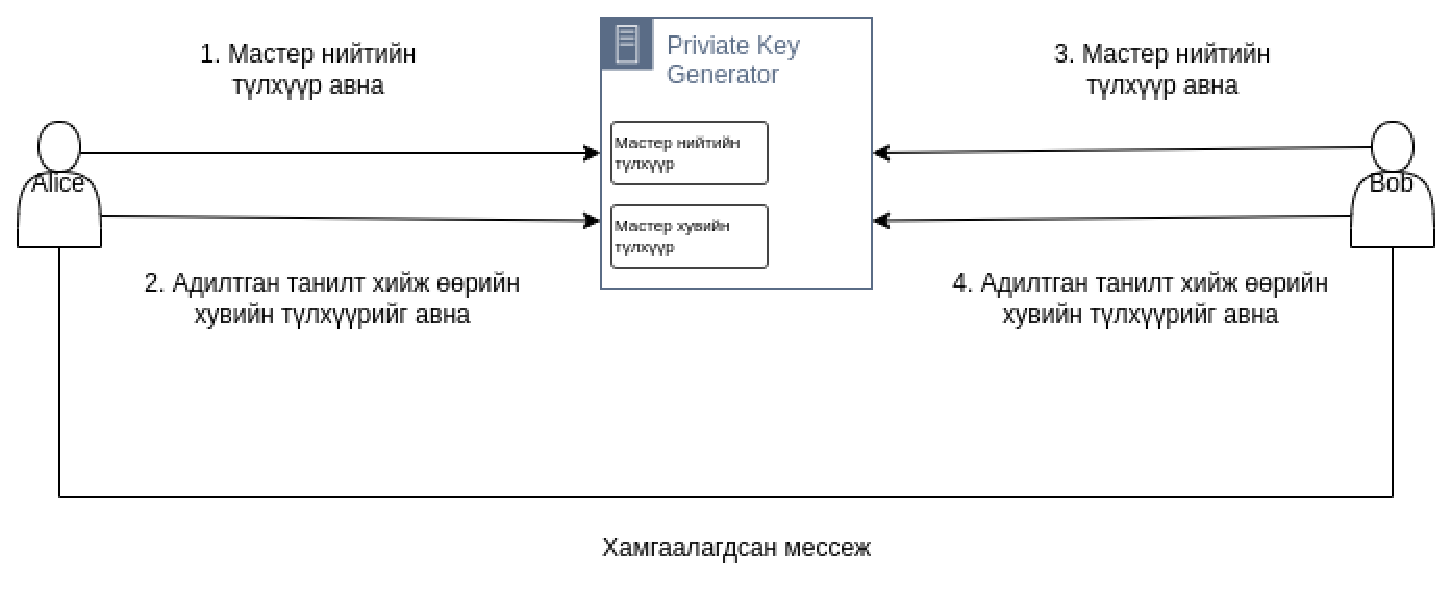
\includegraphics[scale=0.6]{Figures/IBE.eps}
\caption[IBE]{Танилтад суурилсан шифрлэлт}
\label{fig:IBE}
\end{figure}

IBE-дээр суурилсан алгоритмууд

\begin{itemize}
    \item Boneh–Franklin (BF-IBE)
    \item Sakai–Kasahara (SK-IBE)
    \item Boneh–Boyen (BB-IBE)
\end{itemize}

\textbf{Давуу талууд}
\begin{itemize}
    \item Тодорхойгүй олон хэрлэгч үед давуу талтай
    \item Мөн нийтийн түлхүүрийг хэрэглээг халж орлох боломжтой
    \item Мөн цаг минут зэрэг ашиглан хандах эрэхийг нарийн тодорхойлж болно. 
\end{itemize}
\subsection*{Шинж чанарт суурилсан шифрлэлэт (ABE)}
IBE-тэй ерөнхийдөө төстэй. Шинж чанаруудаар бүлэглэж зөвхөн нэг хэрлэгчийн түлхүүр ашиглахгүй олон хүн тайлах боломжтой.
Үндсэн хоёр төрөлтэй. Түлхүүр-Дүрэмийн шинж чанарт суурилсан шифрлэлт (KP-ABE) болон Шифртескт-Дүрэмийн шинж чанарт суурилсан шифрлэлт (CP-ABE).

ABE ерөнхий санаа нь сайн болов ч сул талуудтай.
\begin{itemize}
    \item Түлхүүр зохицуулалт
    \item Түлхүүр хадгалах
    \item Түлхүүр хүчингүй болгох
\end{itemize}

\subsubsection*{KP-ABE}
Хэрэглэгч бүр шинж чанруудтай. Хэрлэгч нь хандалтын модыг өөртөө агуулдаг тул бүх хэрэлэгч өгөгдөл рүү хандах эрхтэй байдаг.
\begin{figure}[ht]
    \centering
    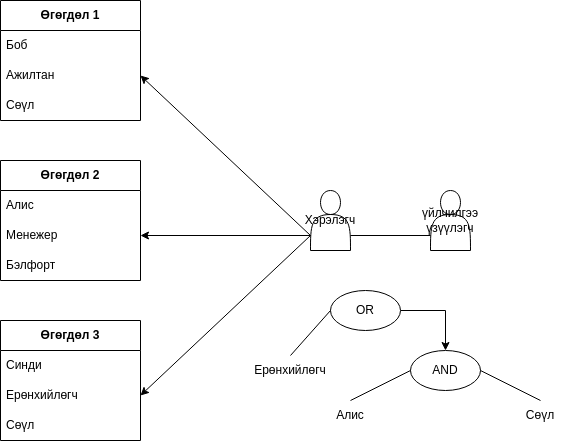
\includegraphics[scale=0.6]{Figures/kp-abe.drawio.png}
    \caption[IBE]{Танилтад суурилсан шифрлэлт}
\label{fig:kp-abe}
\end{figure}

\subsubsection*{CP-ABE}
KP-ABE-ээс ялгаатай зүйл нь шифр нь өрөө хандалтын модыг агуулдаг. KP-ABE-ээс ялгаатай нь шифрлэгдсэн текст нь хандалтын модыг агуулдаг. Хэрэв хэрэглэгчийн шинж чанар нь шифрлэгдсэн текст дэх хандалтын модны нөхцөлийг хангаж байвал шифрлэгдсэн өгөгдлийг тайлах боломжтой. Хандалтын мод нь шифрлэгдсэн өгөгдөлд байгаа тул өгөгдлийн хандалтыг хянах боломжтой.
\begin{figure}[ht]
    \centering
    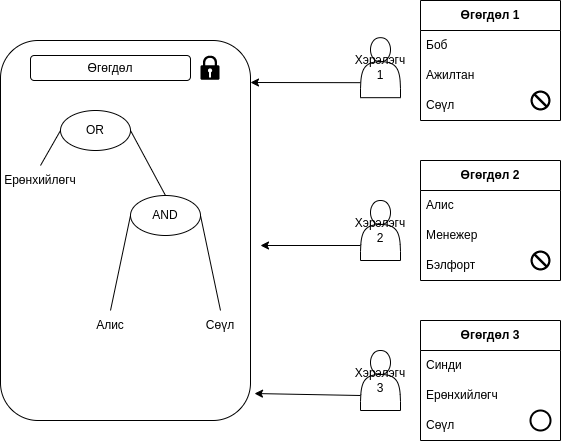
\includegraphics[scale=0.6]{Figures/cp-abe.drawio.png}
    \caption[IBE]{Танилтад суурилсан шифрлэлт}
    \label{fig:cp-abe}
\end{figure}

\subsection*{Гомоморф шифрлэлт (HE)}

Энэ нь шифрлэгдсэн өгөгдлийг тайлахгүйгээр тооцоолол хийх боломжийг олгодог шифрлэлтийн төрөл юм. Аюулгүй үүлэн тооцоолол, цахим санал хураалт, эмнэлгийн бүртгэл гэх мэт төрөл бүрийн хэрэглээнд хэрэглэж болдог.
\cite*{WikiHE}

\begin{itemize}
    \item Хэсэгчилсэн гомоморф шифрлэлт (PHE). PHE-д "хэсэгчилсэн" гэдэг нь зөвхөн сонгосон математик функцийг шифрлэгдсэн утгууд дээр боловсруулах боломжтой. Зөвхөн нэг үйлдлийг нэмэх эсвэл үржүүлэхийг шифрлэгдсэн текст дээр хязгааргүй олон удаа хийхийг зөвшөөрдөг.
    \item Зарим ижил төстэй шифрлэлт (SHE). "Somewhat" нь PHE-ээс илүү ерөнхий шинж чанартай бөгөөд энэ нь нэмэх, үржүүлэх бүхий гомоморф үйлдлийг дэмждэг. Гэхдээ энд байгаа гол сул тал нь зөвхөн цөөн тооны үйлдлийг гүйцэтгэх боломжтой юм.
    \item Бүрэн гомоморфик шифрлэлт (FHE). PHE болон SHE нь хязгаарлагдмал ажиллагаатай бол бүрэн гомоморф шифрлэлт нь шифрлэгдсэн текстэн дээр хязгаарлалтгүйгээр нэмэх болон үржүүлэх үйлдлийг хоёуланг нь ашиглах чадвартай.
\end{itemize}

Хямд үүлэн тооцоолол, үүлэн хадгалах систем нь аж ахуйн нэгжүүд болон хувь хүмүүсийн өгөгдлөө ашиглах, удирдах арга хэлбэрийг үндсээр нь өөрчилсөн. AES гэх мэт уламжлалт шифрлэлтийн аргууд нь маш хурдан бөгөөд өгөгдлийг шифрлэгдсэн хэлбэрээр хялбархан хадгалах боломжийг олгодог. Гэсэн хэдий ч, шифрлэгдсэн өгөгдөл дээр энгийн дүн шинжилгээ хийхийн тулд үүлэн сервер нууц түлхүүрт хандах шаардлагатай бөгөөд энэ нь аюулгүй байдлын асуудалд хүргэдэг, эсвэл өгөгдөл эзэмшигч нь өгөгдлийг татаж авах, тайлах, локал байдлаар ажиллуулах шаардлагатай. зардал ихтэй, логистикийн сорилтыг бий болгоно. Клоуд нь шифрлэгдсэн өгөгдөл дээр шууд ажиллаж, зөвхөн шифрлэгдсэн үр дүнг өгөгдлийн эзэнд буцааж өгөх боломжтой тул гомоморф шифрлэлтийг энэ хувилбарыг ихээхэн хялбарчлахад ашиглаж болно. Хэрэглээний илүү төвөгтэй хувилбарууд нь гуравдагч этгээдийн ажиллах боломжтой хувийн өгөгдөл бүхий олон талуудыг оролцуулж, үр дүнг нэг буюу хэд хэдэн оролцогчид шифрлэхээр буцааж өгч болно.

\textbf{Давуу талууд}
\begin{itemize}
    \item Найдваргүй гуравдагч орчинд өгөгдөл найдвартай, нууцлалтай хэвээр байна. Өгөгдөл нь үргэлж шифрлэгдсэн хэвээр байх бөгөөд энэ нь нууц мэдээлэл алдагдуулах магадлалыг бууруулдаг.
    \item Бүрэн гомоморф шифрлэлтийн схемүүд нь квант халдлагын эсрэг тэсвэртэй.
\end{itemize}

\textbf{Сул талууд}
\begin{itemize}
    \item Тооцооллын хурд багатай 
    \item Нарийвчлал багатай
\end{itemize}
%-------------------------------------------------------------------------------
%	SECTION 4
%-------------------------------------------------------------------------------

\section{Файл шифрлэх хадгалах}

Файлыг тэгш хэмт болон тэгч бус шифрлэлтээр аль алингаар нь шифрлдэг. Тэгш хэмт шифрлэлт нь тэгш бус хэмт шифрлэлтээс хувьд хурдан боловч түлхүүр дамжуулах зэрэгт асуудал үүсдэг.
Ихэвчлэн тэгш бус шифрэлэлтээр файлыг шифрлэдэг ба тэгш хэмт шифрэлтээс илүү хурдан байдаг.

\textbf{Нийтлэг ашигладаг алгоритмууд}
\begin{itemize}
    \item Нарийвчилсан шифрлэлтийн стандарт (AES): AES нь тэгш хэмт шифрлэлтийн алгоритм бөгөөд хамгийн найдвартай гэж тооцогддог.
    \item Гурвалсан өгөгдөл шифрлэлтийн стандарт (3DES): 3DES нь аюулгүй гэж тооцогддог хуучин тэгш хэмтэй шифрлэлтийн алгоритм юм. Энэ нь ихэвчлэн өндөр хамгаалалттай байх шаардлагагүй өгөгдлийг шифрлэхэд ашиглагддаг.
    \item Ривест-Шамир-Адлеман (RSA): RSA нь бусадтай хуваалцах шаардлагатай өгөгдлийг шифрлэхэд ихэвчлэн ашиглагддаг тэгш бус шифрлэлтийн алгоритм юм. Үүнийг мөн тоон гарын үсэг үүсгэхэд ашигладаг бөгөөд үүнийг баримт бичиг эсвэл мессежийн жинхэнэ эсэхийг шалгахад ашиглаж болно.
\end{itemize}

\subsection*{Файлын системийг шифрлэх}
Файл системийн түвшинд шифрлэлтийг файлд суурилсан шифрлэлт (FBE) эсвэл файл/хавтас шифрлэлт гэдэг нэрлдэг дискний шифрлэлтийн нэг төрөл юм.\cite{WikiEnFileSystem}

Файл системийн шифрлэлтийн төрөл
\begin{itemize}
    \item Криптограф файлын систем
    \item Ерөнхий зориулалт бүхий файлын шифрлэлт системүүд
\end{itemize}

Давуу талууд
\begin{itemize}
    \item Файлд суурилсан уян хатан түлхүүрийн удирдлага гэдэг нь файл бүрийг тусдаа түлхүүрээр шифрлэх боломжтой.
    \item Шифрлэгдсэн файлын тус тусд нь удирдах нь шифрлэгдсэн файлыг бүхэлд нь засаж өөрчлөхийн оронд зөвхөн өөрчлөгдсөн хэсгийг л өөрчлөх боломжтой.
    \item Хандалтын нийтийн түлрүүр ашиглах хянах боломжтой.
\end{itemize}

\subsection*{Криптограф файлын систем}

Криптограф файлын системүүд нь шифрлэлт, аюулгүй байдлын үүднээс тусгайлан бүтээгдсэн (ерөнхий зориулалтын бус) файлын системүүд юм. Тэд ихэвчлэн мета өгөгдлийг оруулаад агуулсан бүх өгөгдлийг шифрлэдэг. Диск дээрх формат болон өөрийн блокийн хуваарилалт хийдэггүй одоо байгаа файлын системүүдийн дээр байрладаг.

\subsection*{Ерөнхий зориулалт бүхий файлын шифрлэлт системүүд}

Криптограф файлын систем болон бүрэн дискний шифрлэлтээс ялгаатай нь файлын системийн түвшинд шифрлэлэт хийдэг ерөнхий зориулалтын файлын системүүд юм. Файлын нэр, хэмжээ, өөрчлөлтийн цагийн тэмдэг гэх мэт файлын системийн мета өгөгдлийг ихэвчлэн шифрлэдэггүй.

%-------------------------------------------------------------------------------
%	SECTION 5
%-------------------------------------------------------------------------------

\section{Бүлгийн Дүгнэлт}

Өгөгдөл хуваалцах болон өгөгдөлийн аюулгүй байдлын судалсан. Орчин үеийн шифрлэлтийн схемүүдийн судлаж файл шифрлэх аргуудыг судалсан.

% \pagecolor{Beige}
% Бүлэг 2

\chapter{Прокси дахин шифрлэлтэд суурилсан файл хуваалцах систем} % Зарим нэг зөвлөмж
\label{Chapter2} % Энэ бүлэг рүү ишлэл хийх бол \ref{Chapter2} командыг ашигла 
\pagecolor{white}

%-------------------------------------------------------------------------------
%	SECTION 1
%-------------------------------------------------------------------------------
\section{Прокси дахин шифрлэлт}
Прокси дахин шифрлэлт нь нийтийн түлхүүрээр шифрлэсэн өгөгдлийг дахин шифрлэж өөр хувийн түлхүүрээр тайлах боломжийг олгодог.

Мамбо болон Окамото шифрийг тайлан дараа нь шифрлэх уламжлалт аргыг сайжруулах зорилгоор анх гаргаж ирсэн.

1998 онд Blaze, Bleumer, Strauss (BBS) нар "atomic proxy cryptography" гэсэн ойлголтыг санал болгосон бөгөөд үүнд хагас итгэмжлэгдсэн прокси нь үндсэн энгийн текстийг харалгүйгээр Алисын шифрийг Бобын шифр текст болгон хувиргадаг. El Gamel дээр суурилсан схем ба прокси буюу гуравдагч талийн тусламжтайгаар шифрийг дамжуулах зорилготой. \cite{ateniese2005improved}

Прокси дахин шифрлэлт үйл явц нь гурван хэсгээс тогтоно.
\begin{itemize}
    \item \textbf{Төлөөлөгч:} Прокси дахин шифрлэлт ашиглан шифрийг тайлах эрхээ өөр хүнд шилжүүлэх өгөгдлийн эзэн. Дахин шифрлэлтийн түлхүүр үүсгэж, прокси руу илгээдэг. Төлөөлөгчийг ихэвчлэн “Алис” гэж нэрлэдэг.
    \item \textbf{Орлгоч:} Төлөөлөгчийн шифрийг тайлах эрхтэй хүн. Ихэвчлэн "Боб" гэдэг нэртэй байдаг.
    \item \textbf{Прокси:} Дахин шифрлэх шифрийг дамжуулах гуравдагч тал.
\end{itemize}

\textbf{Прокси дахин шифрлэлт үндсэн хоёр төрөлтэй.}
\begin{itemize}
    \item Нэг чиглэлт (Unidirectional PRE)
    \item Хоёр чиглэлт (Bidirectional PRE)
\end{itemize}
Мөн олон дахин шифрлэх боломжтой болон нэг удаагийн шифрлэх боломжтой гэж хуваадаг.

Прокси дахин шифрлэх схем дараах хэсгүүдээс тогтоно.
\begin{itemize}
    \item \textbf{Нийтийн параметрүүд:} Нийтлэг нийтэд байдаг параметрүүд. Түлхүүрийн урт зэрэг.

    \item \textbf{Нийтийн болон нууц түлхүүрийн хослол:} Хэрэглэгч бүр нийтийн/нууц түлхүүрийг үүсгэдэг. Нийтийн түлхүүрийг нийтэд тавьж, харин хувийн түлхүүр нь зөвхөн хэрэглэгч өөртөө үлдээнэ. Боб Алис руу мессеж илгээхдээ Алисын нийтийн түлхүүрийг ашиглан шифрлэж, Алис түүний хувийн түлхүүрийг ашиглан тайлна.
    
    \item \textbf{Төлөөлөгчийн түлхүүрүүд:} Хэрэглэгч бүр энд rkAlice→Bob гэж тэмдэглэсэн дурын төлөөлөгчид (дахин шифрлэх) түлхүүр үүсгэж болно. rkAlice→Bob тулд Алис прокси дахин шифрлэлтийн алгоритмыг ашиглан хувийн түлхүүрээ Бобын нийтийн түлхүүртэй хослуулан түлхүүр гаргаж авна. Гаргаж авсан түлхүүрээр дахин шифрлэж төлөөлөгчийн хувийн түлхүүрээр тайлах боломжтой болно.
    
    \item \textbf{Шифрлэгдсэн текст:} Хэрэглэгч ямар нэгэн нийтийн түлхүүрээр мессежийг (энгийн текст) шифрлэх үед шифр текст үүснэ.
\end{itemize}

Нэг чиглэлт \emph{PRE (KE, RG, E, R, D)} хэсгүүдээс тогтоно.
\begin{enumerate}
    \item Алис, Боб болон Чарли хувийн болон нийтийн түлхүүрийг үүсгэнэ. \emph{(KE)}
    \item Алис Боб-д зориулж өгөгдлөө шифрлэж серверт байршуулна.
    \item Боб Алис-ын өгөгдлийг Чарли-тай хуваацлахын тулд \emph{RE(pkB,skB,pkC,skC∗)} шифрлэж серверт байршуулна. Чарлигийн хувийн заавал шаардахгүй үүсгэж болно.
    \item Боб RE-г ашиглаж үүсгэсэн түлхүүрийг серверт явуулж Алисын файлыг дахин шифрлэж Чарли тайлах боломжтой болно.
\end{enumerate}

\begin{figure}[ht]
    \centering
    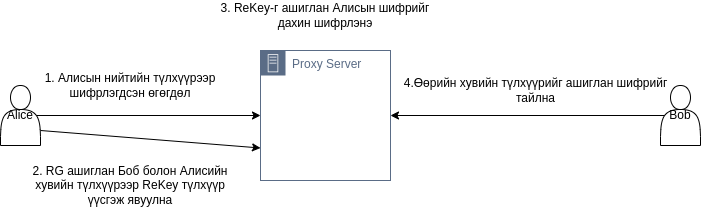
\includegraphics[scale=0.5]{Figures/PRE.drawio.png}
    \caption[Proxy Re-encryption scheme]{Прокси дахин шифрлэх}
    \label{fig:PRE_Scheme}
\end{figure}

Давуу талууд:
\begin{itemize}
    \item Нууцлалыг сайжруулна: PRE нь оролцогч талуудын хувийн мэдээллийг задруулахгүйгээр өгөгдлийг хуваалцахыг зөвшөөрснөөр нууцлалыг сайжруулдаг. Талууд нууцаар эсвэл хувийн нууц мэдээллийг задруулахгүйгээр мэдээллээ хуваалцахыг хүссэн тохиолдолд ашиглах боломжтой.
    \item Илүү уян хатан шифрлэсэн өгөгдлийг өргөн хүрээтэй тараах боломжтой
\end{itemize}

Сул талууд:
\begin{itemize}
    \item Проксид итгэх: PRE нь дахин шифрлэлтийг гүйцэтгэхэд гуравдагч талын прокси дээр тулгуурладаг ба схемийн аюулгүй байдал нь прокси талаас хамаарна.
    \item Хязгаарлагдмал өргөтгөх чадвар: PRE нь өргөтгөх чадварын хувьд хязгаарлагдмал байж болно. Учир нь хэрэглэгчдийн тоо нэмэгдэхийн хэрээр олон талыг дэмжихэд шаардлагатай дахин шифрлэлтийн түлхүүрүүдийн тоо хурдацтай өсөх болно. Энэ нь гол менежментийг төвөгтэй болгож, удирдахад хэцүү болгодог.
    \item Potential for replay attacks: PRE нь халдагч хариуг зогсоож хандах эрхийг өөрт ашигтай солих боломжтой. 
    \item Хүчингүй болгоход хүндрэлтэй: PRE дахь өгөгдөлд хандах эрхийг цуцлах нь ялангуяа олон тал оролцсон тохиолдолд төвөгтэй. Хэрэв аль нэг талын дахин шифрлэлтийн түлхүүр алдагдсан бол бусад талуудын мэдээлэлд хандах эрхэд нөлөөлөхгүйгээр өгөгдөлд хандах эрхийг цуцлах нь хэцүү юм.
    \item Хязгаарлагдмал хэрэглээ: PRE нь харьцангуй шинэ бөгөөд шинээр гарч ирж буй технологи хэвээр байгаа бөгөөд илүү уламжлалт шифрлэлтийн схемүүдтэй харьцуулахад хэрэглээ нь хязгаарлагдмал байдаг. Энэ нь технологийг хэрэгжүүлэх, удирдах туршлагатай мэргэжилтнүүд бага байдаг.
\end{itemize}

\subsection*{Прокси дахин шифрлэх схемийн ерөнхий хэрэглээ}
\begin{itemize}
    \item \textbf{Аюулгүй өгөгдөл хуваалцах:} Өгөгдлийн олон хэрлэгчид найдвартай хуваалцахад ашигладаг. Өгөгдлийн эзэмшигч нь өгөгдлийг өөрийн түлхүүрээр шифрлэж, дахин шифрлэж прокси руу шилжүүлдэг. Дараа нь прокси нь хүлээн авагчийн түлхүүрээр шифрлэгдсэн өгөгдлийг хувиргаж, өгөгдөл эзэмшигчийн оролцоогүйгээр шифрийг тайлж, өгөгдөлд хандах боломжийг олгодог.

    \item \textbf{Cloud Storage:} Үүл хадгалах системд хадгалагдсан мэдээллийн аюулгүй байдлыг сайжруулахын тулд прокси дахин шифрлэлтийг ашиглаж болно. Нууц мэдээллийг үүлэн үйлчилгээ үзүүлэгч рүү шууд оруулахын оронд өгөгдлийг эзэмшигчийн түлхүүрээр шифрлэж, прокси түлхүүрээр дахин шифрлэх боломжтой. Дараа нь прокси нь дахин шифрлэгдсэн өгөгдлийг үүлэн дотор хадгалдаг. Энэ нь үүлэн үйлчилгээ үзүүлэгч нь зөвхөн дахин шифрлэгдсэн өгөгдөлд хандах эрхтэй бөгөөд анхны контентыг уншиж чадахгүй байх боломжийг олгодог.

    \item \textbf{Түлхүүр эскроу:}Түлхүүр эскроу гэдэг нь криптограф түлхүүрийг итгэмжлэгдсэн гуравдагч этгээдэд хадгалах практикийг хэлнэ. Энэ тохиолдолд анхны өгөгдөл нь эзэмшигчийн түлхүүрээр шифрлэгдсэн бөгөөд дахин шифрлэлтийн түлхүүрnийг проксид хадгалагдана. Хэрэв эзэмшигч нь түлхүүрээ алдсан эсвэл өөр төхөөрөмжөөс хандах шаардлагатай бол прокси нь өгөгдлийг шинэ түлхүүрээр дахин шифрлэх боломжтой бөгөөд ингэснээр эзэмшигчид дахин хандах эрх олгоно.

    \item \textbf{Аюулгүй Имэйл Холбоо:} Илгээгч нь хувийн түлхүүрээ шуудангийн сервер эсвэл бусад зуучлагчтай хуваалцахын оронд өөрийн түлхүүрээр имэйлээ шифрлэж, дахин шифрлэх ажиллагааг прокси руу шилжүүлэх боломжтой. Дараа нь прокси нь хүлээн авагчийн түлхүүрээр имэйлийг дахин шифрлэх боломжтой бөгөөд зөвхөн хүлээн авагч нь мессежний кодыг тайлж унших боломжтой.
\end{itemize}

% \subsection*{Прокси дахин шифрлэх схемийн ашиглаж буй системүүд}
% \begin{itemize}
%     \item Google Cloud Platform (GCP) Cloud Түлхүүр Удирдлагын Үйлчилгээ: GCP Үүлэн Түлхүүр Удирдлагын Үйлчилгээ нь үүлэнд суурилсан программууд, гар утасны программууд болон вэб программууд зэрэг төрөл бүрийн программуудын шифрлэлтийн түлхүүрүүдийг хадгалахад ашиглагдаж болно. PRE нь хэрэглэгчдэд шифрлэлтийн түлхүүрийг хуваалцах шаардлагагүйгээр шифрлэгдсэн өгөгдлийг бусадтай хуваалцах боломжийг олгоход ашиглаж болно. Жишээлбэл, компани GCP Cloud Түлхүүр Удирдлагын Үйлчилгээг ашиглан үйлчлүүлэгчийнхээ мэдээллийн шифрлэлтийн түлхүүрүүдийг хадгалах боломжтой. Дараа нь компани PRE-г ашиглан ажилтнууддаа шифрлэлтийн түлхүүрүүдийг ажилчидтайгаа хуваалцахгүйгээр хэрэглэгчийн мэдээлэлд хандах боломжийг олгох боломжтой. Энэ нь ажилтны компьютер эвдэрсэн ч гэсэн хэрэглэгчийн мэдээллийн нууцлалыг хамгаалахад тусална.
% \end{itemize}

%-------------------------------------------------------------------------------
%	SECTION 2
%-------------------------------------------------------------------------------
\section{Хөгжүүлэх технологи, хэл сонгох}
Прокси дахин шифрлэлт схемийг ашиглан файл хуваалцах систем хөгжүүлэхээр болсон.Хөгжүүлэлтэнд хэрэгтэй хэл болон технологи сонгосон.

Систем хоёр хэсгээс тогтох ба. API сервер болон хэрлэгч талын программ. Пайтон маш олон нэмэлт сангууд байдаг маш том нийгэмлэгтэй (community) хэл. Бичиглэл хялбар олон давуу талтай тул пайтон хэлийг сонгосон.
Үүнд:
\subsubsection*{\textbf{Flask framework}}
Пайтон хэл дээр бичсэн веб хөгжүүлэхэд зориулагдсан  фреймворк юм. Хөнгөхөн олон нэмэлт сан шаардахгүй хэрэгтэй сангуудаа суулгаад хөгжүүлэх боломжтой. Сурахад хялбар өөрийн хүссэн загвараар загварчилж хийх боломжтой. RESTFul API гаргахад хялбар. Хэрэгтэй гэвэл нэмэлт сан ORM зэрэг өөр сангууд суулгаж хамт ашиглах боломжтой.
\begin{lstlisting}[language=Python]
from flask import Flask

app = Flask(__name__)
        
@app.route("/")
    def hello_world():
        return "<p>Hello, World!</p>"
@app.get("/")
    def hello_world():
        return "<p>Hello, get request!</p>"
\end{lstlisting}
app.route endpoint бичих боломжтой маш хялбар мөн хурдан бичих боломжтой. 
\subsubsection*{\textbf{Tkinter}}
Хэрэглэгчийн интерфейс (GUI) үүсгэхэд ашигладаг Python номын сан юм. Tcl/TK GUI дээр суурилсан. Линукс виндовс зэрэг олон үйлдлийн системийг дэмждэг. Нэмэлт сангуудтай ажиллах боломжтой.
\begin{lstlisting}[language=Python]
import tkinter as tk

root = tk.Tk()
# Create a label widget.
label = tk.Label(root, text="Hello, world!")
# Create a button widget.
button = tk.Button(root, text="Click me!")
# Add the label and button widgets to the root window.
label.pack()
button.pack()
# Start the main loop.
root.mainloop()
\end{lstlisting}
Энгийн бичхэд хялбар нийгэмлэг сайн.
\subsubsection*{\textbf{pyUmbral}}
Прокси дахин шифрлэлтийг файтон дээр хэрэгжүүлсэн пайтоны сан юм. OpenSSL болон Cryptography.io ашиглсан.
\begin{figure}[ht]
    \centering
    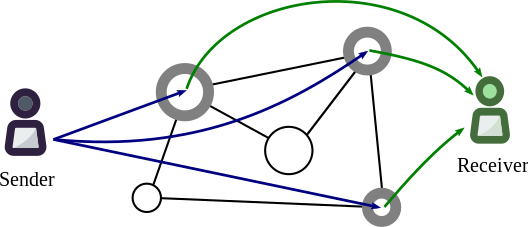
\includegraphics[scale=0.5]{Figures/umbral.png}
    \caption[pyUmbral]{pyUmbral}
    \label{fig:pyUmbral}
\end{figure}

ECIES-KEM болон BBS98 санаа авсан нэг чиглэлтэй дахин шифрлэлтийн сан. pyUmbral функцуудийг ерөнхийд нь гурав ангилсан.
\begin{enumerate}
    \item Түлхүүр үүсгэх алгоритмууд.
    \begin{itemize}
        \item KeyGen()
        \item ReKeyGen(skA, pkB, N, t)
    \end{itemize}
    \item Encapsulation болон Decapsulation
    \begin{itemize}
        \item Encapsulate(pkA)
        \item Decapsulate(skA, capsule)
    \end{itemize}
    \item Re-Encapsulation болон Fragments Decapsulation.
    \begin{itemize}
        \item ReEncapsulation(kF rag, capsule)
        \item DecapsulateFrags(skB, {cF ragi}ti=1, capsule):
    \end{itemize}
\end{enumerate}

\subsubsection*{\textbf{Google Cloud Platform}}
Гуравдагч тал болох сервер проксиг (API) deploy хийж байршуулах шаардлагатай0. Google Cloud нь маш олон давуу талтай ба үнэгүй туршиж үзэх 300 долларын эрхтэй тул сонгосон.

%-------------------------------------------------------------------------------
%	SECTION 3
%-------------------------------------------------------------------------------
\section{Хөгжүүлэлтийн орчин бэлдэх}
Пайтон хэл нь орчин бүрдүүлэхэд хялбар ба виртуал орчин үүсгэж хэрэгтэй сангуудыг татаж суулгах боломжтой. Бүх линукс тархцад пайтон хэл нь суулгалцан байдаг тул хэрэгтэй сангуудыг татаж суулгахад л хангалтай. 

Пайтон хэл дээр хөгжүүлэлт хийхийн тулд прокси дахин шифрлэлтийн пайтон дээр сан бичих гэж оролдож үзсэн.
JHU-MIT Proxy Re-cryptography Library (PRL) нь хэд хэдэн прокси дахин шифрлэлтийн схемийг хэрэгжүүлсэн нээлттэй эхтэй сан юм. Алгоритмуудыг Жонс Хопкинсийн Их Сургууль болон Массачусетсийн Технологийн Их Сургуулийн судлаачид боловсруулсан бөгөөд Жузеппе Атениезе, Кевин Фу, Мэттью Грин, Сюзан Хохенбергер нарын анхны судалгаанд үндэслэсэн. 
JHU-MTI Прокси дахин шифрлэлтийн сан нь C/C++ хэл дээр бичигдсэн байсан. Пайтон хэлний setuptools болон C хэлний "python.h" санг ашиглан пайтоны сан бичих гэж оролдож үзсэн. JHU-MTI сан нь MIRCL санг ашигладаг.

PRL сан нь хоёр схемийг хэрэгжүүлдэг.
\begin{itemize}
    \item \textbf{PRE1:} алгоритм нь Decisional Billinear Diffie-Hellman Assumption (DBDH) дагуу аюулгүй.
    \item \textbf{PRE2:} алгоритм нь Decisional Billinear Inversion Assumption (DBDHI)-ийн дагуу аюулгүй.
\end{itemize}

PRE1 схемийг пайтон сан руу хөрвүүлэх гэж оролдсон.\\
\textbf{Ерөнхий бүтэц}
\dirtree{%
.1 ..
.2 example.
.3 example.py.
.2 external.
.3 miracl.
.3 proxylib.
.2 LICENSE.
.2 README.md.
.2 setup.py.
.2 src.
.3 pypre.cpp.
.2 userguide.pdf.
}\\
\begin{itemize}
    \item \textbf{example} хэсэг тестийн код байрлана.
    \item \textbf{external} хэсэгт PRL сан болон MIRCL сан байна.
    \item Сангуудыг compile хийж \textbf{lib*.a} файл гаргаж авна.
    \item \textbf{setup.py} файл нь тухайн package-ын мэдээлэл байна.
    \item \textbf{pypre.cpp} С++ функцийг нэмэлт сан *.a-аас дуудаж пайтон руу хөрвүүлэх хэсэг. 
\end{itemize}

\begin{lstlisting}[language=Python, caption={setup.py}]
import glob
import os

from setuptools import Extension, setup

os.environ["CC"] = "g++"
os.environ["CXX"] = "g++"

module = Extension(
    "pypre",
    language="c++",
    sources=[f for f in glob.glob('src/*.cpp')]+
    ['external/proxylib/proxylib_pre1.cpp'],
    include_dirs=["external/miracl", "external/proxylib"],
    library_dirs=["external/miracl", "external/proxylib"],
    libraries=["miracl", "proxylib"],
    extra_objects=['external/miracl/libmiracl.a','external/proxylib/libproxylib.a']
)

setup(name='pypre',
      license='Apache',
      author="Myagmartseren",
      author_email='myagmartseren7@gmail.com',
      description='Proxy Re-encryption Python library',
      url='https://github.com/myagmartseren/pre_python',
      ext_modules=[module],
      include_dirs=['external/proxylib','external/miracl'],
)
\end{lstlisting}

\textbf{pypre.py} файл дотор үндсэн C++ кодны санг дуудаж пайтонруу хөрвүүлэх хэсэг байна. 
Хэрэгтэй толгой файлыг include хийнэ. Proxylib.h болон miracle гэх мэт сангууд нь setup.py хавсарсан сангууд юм.

\begin{lstlisting}[language=C, caption={setup.py}]
#define PY_SSIZE_T_CLEAN
#include <zzn.h>
#include <miracl.h>

#include <Python.h>
#include <proxylib.h>
#include <proxylib_pre1.h>    
\end{lstlisting}

\noindent Class бүрийг C-ын struct-ыг ашиглаж зарлаж өгнө. Class-ын method-уудыг мөн адил зарлаж өгнө. 

\begin{lstlisting}[language=C, caption={setup.py}]
typedef struct
{
    PyObject_HEAD
    ProxyCiphertext_PRE1 *proxyCiphertext_PRE1;
} PyProxyCiphertext_PRE1;

static PyObject* PyPRE1_generate_params(PyObject *self, PyObject *args) {
    if (PyTuple_Size(args) !=1){
        PyErr_SetString(PyExc_RuntimeError, "Should have CurveParams");
        return Py_None;
    }

    PyObject *params = PyTuple_GetItem(args, 0);

    if (!PyCurveParams_Check(params)) {
        PyErr_SetString(PyExc_RuntimeError, "Failed to cast CurveParams");
        return Py_None;
    }

    PyCurveParams *pyParams = (PyCurveParams *)params;

    int result = PRE1_generate_params(*pyParams->params);
    if (!result) {
        PyErr_SetString(PyExc_RuntimeError, "Failed to generate params");
        return PyBool_FromLong(result);
    }

    Py_INCREF(Py_None);
    return PyBool_FromLong(result);
}

static PyObject* PyPRE1_keygen(PyObject *self, PyObject *args) {
    if (PyTuple_Size(args) !=3){
        PyErr_SetString(PyExc_RuntimeError, "Should have 3 parameters");
        return Py_None;
    }

    PyObject *tempParams = PyTuple_GetItem(args, 0);
    if (!PyCurveParams_Check(tempParams)) {
        PyErr_SetString(PyExc_RuntimeError, "Failed to cast CurveParams");
        return Py_None;
    }
    PyCurveParams *pyParams = (PyCurveParams *)tempParams;
    printf("pyParams->params address: %p\n", pyParams->params);

    PyObject *tempPublicKey = PyTuple_GetItem(args, 1);
    if (!PyProxyPK_PRE1_Check(tempPublicKey)) {
        PyErr_SetString(PyExc_RuntimeError, "Failed to cast PK_PRE1");
        return Py_None;
    }
    PyProxyPK_PRE1 *pyPublicKey = (PyProxyPK_PRE1 *)tempPublicKey;
    printf("pyPublicKey->publicKey address: %p\n", pyPublicKey->publicKey);

    PyObject *tempSecretKey = PyTuple_GetItem(args, 2);
    if (!PyProxySK_PRE1_Check(tempSecretKey)) {
        PyErr_SetString(PyExc_RuntimeError, "Failed to cast SK_PRE1");
        return Py_None;
    }
    PyProxySK_PRE1 *pySecretKey = (PyProxySK_PRE1 *)tempSecretKey;
    printf("pySecretKey->secretKey address: %p\n", pySecretKey->secretKey);

    int result = PRE1_keygen(*pyParams->params, *pyPublicKey->publicKey, *pySecretKey->secretKey);
    
    Py_INCREF(Py_None);
    return PyBool_FromLong(result);
}

static PyMethodDef module_methods[] = {
    {"PRE1_generate_params", PyPRE1_generate_params, METH_VARARGS, "Generate curve parameters for the PRE1 scheme."},
    {"PRE1_keygen", PyPRE1_keygen, METH_VARARGS, "Generate curve parameters for the PRE1 scheme."},

    {NULL, NULL, 0, NULL}
};
\end{lstlisting}
\noindent Классуудыг модулд нэмж өгнө. Мөн статик функцуулийг нэмж өгнө.

\begin{lstlisting}[language=C, caption={setup.py}]
static struct PyModuleDef module_def = {
    PyModuleDef_HEAD_INIT,
    "pypre",
    0,  // m_doc
    -1, // m_size
    module_methods,// m_methods
    /*
    NULL,                 // m_reload
    NULL,                 // m_traverse
    NULL,                 // m_clear
    NULL                  // m_free
    */
};

PyMODINIT_FUNC PyInit_pypre(void);

PyObject *PyInit_pypre(void)
{
    extern PyTypeObject PyCurveParamsType;
    if (PyType_Ready(&PyCurveParamsType) < 0)
        return NULL;

    PyObject *module = PyModule_Create(&module_def);

    Py_INCREF(&PyCurveParamsType);
    if (PyModule_AddObject(module, "CurveParams", (PyObject *)&PyCurveParamsType) < 0)
    {
        Py_DECREF(&PyCurveParamsType);
        Py_DECREF(module);
        return NULL;
    }

    extern PyTypeObject PyProxyPK_PRE1Type;
    if (PyType_Ready(&PyProxyPK_PRE1Type) < 0)
        return NULL;

    Py_INCREF(&PyProxyPK_PRE1Type);
    if (PyModule_AddObject(module, "PK_PRE1", (PyObject *)&PyProxyPK_PRE1Type) < 0)
    {
        Py_DECREF(&PyProxyPK_PRE1Type);
        Py_DECREF(module);
        return NULL;
    }

    extern PyTypeObject PyProxySK_PRE1Type;
    if (PyType_Ready(&PyProxySK_PRE1Type) < 0)
        return NULL;

    Py_INCREF(&PyProxySK_PRE1Type);
    if (PyModule_AddObject(module, "SK_PRE1", (PyObject *)&PyProxySK_PRE1Type) < 0)
    {
        Py_DECREF(&PyProxySK_PRE1Type);
        Py_DECREF(module);
        return NULL;
    }
    // PyModule_AddObject(module, "__version__", PyUnicode_FromString(VERSION));

    if (PyErr_Occurred())
        PyErr_SetString(PyExc_ImportError, "pypre: init failed");

    return module;
}
\end{lstlisting}

\noindent PRE1 хөрвүүлж байсан боловч цаг хугацааны хувьд амжихгүй болсон тул pyUmbral санг ашиглахаар шийдсэн.

%-------------------------------------------------------------------------------
%	SECTION 4
%-------------------------------------------------------------------------------
\section{Бүлгийн дүгнэлт}
Прокси дахин шифрлэлт судлаж системийг хөгжүүлэлтэнд шаардлагатай технологиуд сангуудыг судлаж хөгжүүлэлт хийж эхэлсэн.
% \pagecolor{Beige}
% Бүлэг 1

\chapter{Прокси дахин шифрлэлтэд суурилсан файл хуваалцах систем хөгжүүлэх}

\label{Chapter3} % Энэ бүлэг рүү ишлэл хийх бол \ref{Chapter1} командыг ашигла 
\pagecolor{white}

%-------------------------------------------------------------------------------
%	SECTION 1
%-------------------------------------------------------------------------------
\section{Системийн шаардлага}
Систем нь түлхүүр үүсгэх файл хадгалах сервер, өгөгдөл эзэмшигч, өгөгдөл хэрэглэгч гэсэн үндсэн гурван хэсгээс тогтоно. Өгөгдөл эзэмшигч бүртгэл үүсгэж өөрийн нийтийн түлхүүр болон хувийн түлхүүрийг үүсгэж авна. Файл шифрлэх болон тайлах үйлдлийг өөрийн төхөөрөмж дээр үйлдэнэ.

\textbf{Системийн оролцогч}
\begin{itemize}
    \item Хэрэглэгч
\end{itemize}

\textbf{Системийн тоглогч}
\begin{itemize}
    \item Файл эзэмшигч
    \item Файл хэрэглэгч
\end{itemize}

\subsection*{Функцийн шаардлага}
Файл эзэмшигчийн функционал шаардлага:
\begin{itemize}
    \item Системд өөрийн бүртгэлийг үүсгэх
    \item Файл оруулах, шифрлэх
    \item Файлыг тайлах хэрлэгч сонгох
    \item Шифрлэсэн файлыг хуваалцсан хэрлэгчдийн жагсаалт
\end{itemize}
Файл хэрэглэгчийн функционал шаардлага:
\begin{itemize}
    \item Системд өөрийн бүртгэлийг үүсгэх
    \item Өөрт хуваацлсан файлын жагсаалт
    \item Файлыг татаж авах
    \item Шифрлэсэн файлыг тайлах
\end{itemize}

\subsection*{Функцийн бус шаардлага}
\begin{enumerate}
    \item Файлыг шифрлэх, шифрийг тайлах хурдан гүйцэтгэдэг байх
    \item Хэрэглэгчийн интерфейс ойлгомжтой энгийн байх.
    \item Прокси серверт файлыг шифрлэсэн байдлаар хадгалах, хуваалцах
    \item Өөрийн бүртгэлийг ашиглаж нэвтрэх
    \item Хувийн түлхүүрийг хэрлэгчийн төхөөрөмж дээр авч явах
\end{enumerate}

\subsection*{Юзкейс диаграмм}
Системийн хэрлэгчид ямар үйлдлүүдийг системд хийж болохыг харуулсан хэрэглээний диаграммыг харууллаа.
\begin{figure}[ht]
    \centering
    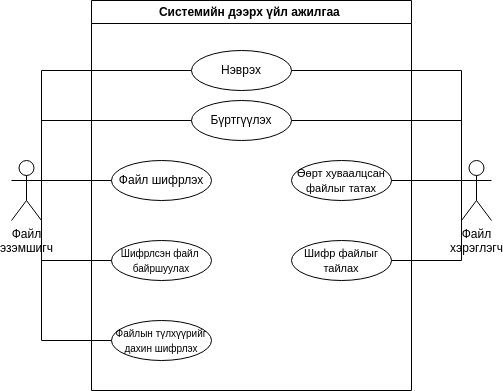
\includegraphics[scale=0.6]{Figures/usecase.drawio.png}
    \caption[Usecase diagram]{Юзкейс диаграмм}
    \label{fig:usecase}
\end{figure}
\subsection*{Юзкейс тодорхойлолт}

\begin{table}
    \label{tab:treatments}
    \footnotesize
    \centering
    \begin{tabularx}{\textwidth}{|>{\hsize=0.3\hsize}X|>{\hsize=0.7\hsize}X|}
        \hline
        \multicolumn{2}{|c|}{Бүртгүүлэх} \\
        \hline
        ID & 1 \\
        \hline
        Үндсэн тоглогч & Файл эзэмшигч болон файл хэрэглэгч\\
        \hline
        Тодорхойлолт & Хэрэглэгч шинээр бүртгэл үүсгэх\\
        \hline
        Өмнөх нөхцөл & Шинэ хэрлэгч байх\\
        \hline
        Үндсэн урсгал & Хэрэглэгчийн мэдээллийг авч өгөгдлийн санд шинэ хэрэглэгч үүсгэх\\
        \hline
        Дараах нөхцөл & Хэрэглэгч өөрийн бүртгэлтэй болох нэвтрэх боломжтой болох\\
        \hline
    \end{tabularx}
    \caption{Бүртгүүлэх юзкейсийн тодорхойлолт}
\end{table}

\begin{table}
    \label{tab:treatments}
    \footnotesize
    \centering
    \begin{tabularx}{\textwidth}{|>{\hsize=0.3\hsize}X|>{\hsize=0.7\hsize}X|}
        \hline
        \multicolumn{2}{|c|}{Нэвтрэх} \\
        \hline
        ID & 2\\
        \hline
        Үндсэн тоглогч & Файл эзэмшигч болон файл хэрэглэгч\\
        \hline
        Тодорхойлолт & Системд нэвтрэх\\
        \hline
        Өмнөх нөхцөл & Бүргэлтэй хэрлэгч байх\\
        \hline
        Үндсэн урсгал & Хэрлэгчийн нууц үг бүртгэл таарч байгааг шалган нэвтрүүлэх\\
        \hline
        Дараах нөхцөл & Бусад хэрэглээ рүү хандах боломжтой болох\\
        \hline
    \end{tabularx}
    \caption{Нэвтрэх юзкейсийн тодорхойлолт}
\end{table}

\begin{table}
    \label{tab:treatments}
    \footnotesize
    \centering
    \begin{tabularx}{\textwidth}{|>{\hsize=0.3\hsize}X|>{\hsize=0.7\hsize}X|}
        \hline
        \multicolumn{2}{|c|}{Файл шифрлэх} \\
        \hline
        ID & 3 \\
        \hline
        Үндсэн тоглогч & Файл эзэмшигч\\
        \hline
        Тодорхойлолт & Файл эзэмшигч файлыг шифрлэх\\
        \hline
        Өмнөх нөхцөл & Систем нэвтэрсэн байх\\
        \hline
        Үндсэн урсгал &
            \item Файлыг сонгох
            \item Санамсаргүй байдлаар түлхүүр үүсгэх
            \item Файлыг тухайн түлхүүрээр шифрлэх
        \\
        \hline
        Дараах нөхцөл & Тухайн төхөөрөмж дээр шифрлэгдсэн байх\\
        \hline
    \end{tabularx}
    \caption{Файл шифрлэх юзкейсийн тодорхойлолт}
\end{table}

\begin{table}
    \label{tab:treatments}
    \footnotesize
    \centering
    \begin{tabularx}{\textwidth}{|>{\hsize=0.3\hsize}X|>{\hsize=0.7\hsize}X|}
        \hline
        \multicolumn{2}{|c|}{Шифрлэсэн файл серверт байршуулах} \\
        \hline
        ID & 4 \\
        \hline
        Үндсэн тоглогч & Файл эзэмшигч\\
        \hline
        Тодорхойлолт & Шифрлэсэн файлыг серверт хуулна\\
        \hline
        Өмнөх нөхцөл & Файлыг шифрэлсэн байх\\
        \hline
        Үндсэн урсгал &
            \item Шифрлэсэн файлыг серверт илгээж
            \item Файлын мэдээллийг өгөгдлийн санд нэмэх 
        \\
        \hline
        Дараах нөхцөл & Файлын талаар мэдээллийг авах боломжтой болох\\
        \hline
    \end{tabularx}
    \caption{Шифрлэсэн файл серверт байршуулах юзкейсийн тодорхойлолт}
\end{table}

\begin{table}
    \label{tab:treatments}
    \footnotesize
    \centering
    \begin{tabularx}{\textwidth}{|>{\hsize=0.3\hsize}X|>{\hsize=0.7\hsize}X|}
        \hline
        \multicolumn{2}{|c|}{Файл хуваалцах} \\
        \hline
        ID & 5 \\
        \hline
        Үндсэн тоглогч & Файл эзэмшигч\\
        \hline
        Тодорхойлолт & Файл эзэмшигч файл хуваалцах хүнийг сонгох\\
        \hline
        Өмнөх нөхцөл & Файлыг серверт байршуулсан байх\\
        \hline
        Үндсэн урсгал &
            \item Файл хуваалцах хүний нийтийн түлхүүрийг авах
            \item Дахин шифрлэх түлхүүр үүсгэх
            \item Файлыг дахин шифрлэх\\
        \hline
        Дараах нөхцөл & Шифрлэсэн файлыг төхөөрөмж дээр тайлхда бэлэн болох\\
        \hline
    \end{tabularx}
    \caption{Файл хуваалцах юзкейсийн тодорхойлолт}
\end{table}

\begin{table}
    \label{tab:treatments}
    \footnotesize
    \centering
    \begin{tabularx}{\textwidth}{|>{\hsize=0.3\hsize}X|>{\hsize=0.7\hsize}X|}
        \hline
        \multicolumn{2}{|c|}{Файл татах} \\
        \hline
        ID & 6 \\
        \hline
        Үндсэн тоглогч & Файл хэрэглэгч\\
        \hline
        Тодорхойлолт & Дахин шифрлэсэн файлыг татаж авах\\
        \hline
        Өмнөх нөхцөл & Файлыг хуваалцсан байх\\
        \hline
        Үндсэн урсгал & Файлыг татаж авах\\
        \hline
        Дараах нөхцөл & Файлыг тайлхад бэлэн болох\\
        \hline
    \end{tabularx}
    \caption{Файл татах юзкейсийн тодорхойлолт}
\end{table}

\begin{table}
    \label{tab:treatments}
    \footnotesize
    \centering
    \begin{tabularx}{\textwidth}{|>{\hsize=0.3\hsize}X|>{\hsize=0.7\hsize}X|}
        \hline
        \multicolumn{2}{|c|}{Шифрлэсэн файлын тайлах} \\
        \hline
        ID & 7 \\
        \hline
        Үндсэн тоглогч & Файл хэрэглэгч\\
        \hline
        Тодорхойлолт & Татаж авсан шифрлэсэн файлыг тайлах\\
        \hline
        Өмнөх нөхцөл & Файлыг хуваалцсан байх\\
        \hline
        Үндсэн урсгал & 
        \item Файлын түлхүүрийг өөрийн хувийн түлхүүрээр тайлах
        \item Файлын түлхүүрээр файлыг тайлах\\
        \hline
        Дараах нөхцөл & Файлыг унших боломжтой болгох\\
        \hline
    \end{tabularx}
    \caption{Шифрлэсэн файлын тайлах юзкейсийн тодорхойлолт}
\end{table}

%-------------------------------------------------------------------------------
%	SECTION 2
%-------------------------------------------------------------------------------
\section{Системийн загвар}

\subsection*{Үйл ажилгааны диаграмм}

\subsection*{Өгөгдлийн сангийн бүтэц}

%-------------------------------------------------------------------------------
%	SECTION 3
%-------------------------------------------------------------------------------
\section{Системийн хөгжүүлэх}

%-------------------------------------------------------------------------------
%	SECTION 4
%-------------------------------------------------------------------------------
% \section{Файл хуваалцах системийг турших}

%-------------------------------------------------------------------------------
%	SECTION 5
%-------------------------------------------------------------------------------

% \section{Дүгнэлт}


%\pagecolor{Beige}
% %----------
%	CONCLUSION OF THESIS
%---------------------------------------------------------------------------------
%\chapter{Дүгнэлт}

\addchaptertocentry{Дүгнэлт}
\pagecolor{white}

%\begin{page}
\section*{\centering \huge{Дүгнэлт}}


 Энд дүгнэлтээ бичнэ. 

%\end{page}


%-------------------------------------------------------------------------------
%	THESIS CONTENT - APPENDICES
%-------------------------------------------------------------------------------

\appendix % Дараах "chapters" нь Хавсралт болохыг LaTex -д хэлэх
% Тезисийн бүлгүүдийг Appendices хавтаснаас бие даасан файл байдлаар оруулах
% \pagecolor{beeige}
% % Хавсралт A

\chapter{Хавсралтын нэр} % Main appendix title

\label{AppendixA} % For referencing this appendix elsewhere, use \ref{AppendixA}
\pagecolor{white}
Хавсралтыг эндээс эхэлж бичнэ. 

% \pagecolor{beeige}
% \chapter{LED контроллер AT89C51ED2} % Main appendix title

\label{AppendixB} % For referencing this appendix elsewhere, use \ref{AppendixA}
\pagecolor{white}
% \pagecolor{beeige}
% \chapter{Хавсралтын нэр} % Main appendix title

\label{AppendixC} % For referencing this appendix elsewhere, use \ref{AppendixA}
\pagecolor{white}

Хавсралтыг эндээс эхэлж бичнэ. 

%-------------------------------------------------------------------------------
%	BIBLIOGRAPHY
%-------------------------------------------------------------------------------
\defformat % Бүлгийн нэрийг оргиналь байдлаар хэвлэх

\addchaptertocentry{Ном зүй} % Ном зүйг гарчигт нэмэх

\printbibliography[heading=bibliography,title={Ном зүй}]

%-------------------------------------------------------------------------------
\end{document}  
 